% main.tex — NeurIPS 2026 submission (official template)
\documentclass{article}
\usepackage{neurips_2026}

\usepackage[utf8]{inputenc}
\usepackage[T1]{fontenc}
\usepackage{amsmath,amssymb}
\usepackage{amsfonts}
\usepackage{graphicx}
\usepackage{booktabs}
\usepackage{multirow}
\usepackage{hyperref}
\usepackage{url}
\usepackage{nicefrac}
\usepackage{microtype}
\usepackage{xcolor}
\usepackage{enumitem}

\title{Spectral Optimization Across Vision Architecture Families:\\A Controlled Empirical Study}

\author{
  Anonymous Author(s)
}

\begin{document}

\maketitle

\begin{abstract}
Optimizer performance in vision models depends critically on architecture: SGD collapses to below 12\% accuracy on layer-normalized architectures while achieving 70\% on batch-normalized ones, a gap that hyperparameter tuning cannot close.
We conduct a controlled empirical study of spectral optimizers---Muon, SOAP, and Shampoo---which exploit weight-matrix spectral structure through Newton-Schulz iteration or Kronecker-factored preconditioning, evaluating them across three architecture families (ResNet-50, DeiT-S, ConvNeXt-T), three datasets, and two training horizons.
The spectral advantage is a \emph{family-level} property: on CIFAR-100---the only dataset where all three were evaluated---all outperform AdamW by +9 to +16\,pp. Muon, tested across all three datasets, maintains gaps of +5.9 to +24.3\,pp.
This advantage is architecture-dependent---largest on layer-normalized networks---and persists across extended training schedules, though gap narrowing varies by architecture. Layer-wise analysis reveals distinct mechanisms: stable-rank divergence correlates positively with optimizer benefit on CNNs ($\rho{=}+0.45$) but negatively on transformers ($\rho{=}{-}0.40$).
A normalization-swap experiment on ResNet-50 provides causal evidence that normalization type mediates the spectral advantage.
\end{abstract}


\section{Introduction}
\label{sec:introduction}

Modern vision architectures have diverged rapidly in structural design: vision transformers use layer normalization and global self-attention~\cite{touvron2021training}, hybrid architectures combine depthwise separable convolutions with layer normalization~\cite{liu2022convnet}, while classical CNNs retain batch normalization~\cite{he2016deep}. Yet optimizer selection has not adapted accordingly---practitioners still default to AdamW or SGD regardless of these structural differences, treating optimizer choice as secondary to architecture and data.

This neglect is consequential. SGD collapses to $11.51\%$ accuracy on layer-normalized ConvNeXt-T while achieving $69.50\%$ on batch-normalized ResNet-50, suggesting normalization type as a critical factor---a hypothesis we examine in Section~\ref{sec:spectral_analysis}. The same task remains accessible to other optimizers, revealing that the optimizer-architecture interaction is not a minor hyperparameter issue but a fundamental compatibility constraint that current practice ignores.

Why do some optimizers transfer across architectures while others fail on certain architectures? Existing first-order methods---AdamW with diagonal curvature estimates, SGD with raw gradient direction---do not explicitly account for how architectural design reshapes the spectral properties of weight gradients. Prior optimizer comparisons typically evaluate single architectures~\cite{schmidt2021crowdedvalley} or lack controlled protocol isolation~\cite{choi2020optimizers}, making it impossible to disentangle optimizer capability from recipe engineering.

We hypothesize that optimizers exploiting \emph{weight-matrix spectral structure}---through Newton--Schulz orthogonalization or Kronecker-factored preconditioning~\cite{bernstein2024old}---should exhibit architecture-robust performance precisely because they adapt to the spectral geometry regardless of how normalization and layer composition reshape it. We test this through a controlled study of three spectral optimizers (Muon~\cite{jordan2024muon}\footnote{At the time of writing, the Muon reference is a blog post and has not been peer-reviewed.}, SOAP~\cite{vyas2024soap}, Shampoo~\cite{gupta2018shampoo}) against AdamW~\cite{loshchilov2019decoupled} and SGD, spanning three architecture families, three datasets, and two training horizons, with independently tuned learning rates per optimizer--architecture pair (Section~\ref{sec:optim_protocol}).

Our experiments confirm the family-level hypothesis across all tested configurations, revealing architecture-dependent mechanisms.

While BOCB~\citep{li2024bocb} diagnoses coupling bias and Kunstner et al.\ explain why SGD fails on transformers~\citep{kunstner2024noise}, neither tests spectral methods nor identifies the architectural mediator. Our work bridges these lines: we evaluate the spectral family that Bernstein \& Newhouse unified theoretically, and identify normalization---not architecture topology---as the mechanism that determines when spectral preconditioning helps.

\paragraph{Contributions.}
\begin{itemize}[leftmargin=*,nosep]
\item The first controlled empirical test of whether Bernstein \& Newhouse's theoretical family~\cite{bernstein2024old} shares practical properties, revealing that normalization type---not architecture family---is the primary mediator of optimizer-architecture coupling.
\item Causal evidence that the spectral advantage is mediated by normalization type: replacing BatchNorm with LayerNorm on ResNet-50 collapses AdamW by ${\sim}17$\,pp while Muon is preserved (+1.64\,pp), and layer-wise stable-rank-divergence correlations reverse sign between CNNs ($\rho{=}{+}0.45$) and transformers ($\rho{=}{-}0.40$).
\item Practical guidance: spectral methods are architecture-robust candidates across the training conditions tested, achieving superior accuracy at substantially lower training cost.
\item A corruption robustness evaluation on CIFAR-100-C showing that spectral optimizers, particularly Muon, improve not only clean accuracy but also robustness to common input corruptions (mCE 89--93\% on three of four architecture configurations vs.\ AdamW baseline of 100\%).
\end{itemize}


\section{Related Work}
\label{sec:related_work}

\paragraph{Optimizer--architecture coupling.}
The observation that optimizer performance depends on architecture is well-established but poorly addressed. SGD dominated the convolutional era~\cite{he2016deep} but fails on modern layer-normalized architectures~\cite{liu2022convnet,touvron2021training}, driving a wholesale shift to AdamW~\cite{loshchilov2019decoupled}. Large-scale benchmarks confirm that no single optimizer dominates across architectures~\cite{choi2020optimizers,schmidt2021crowdedvalley,dahl2024benchmarking}, and Li et al.~\cite{li2024bocb} formalize this as \emph{backbone--optimizer coupling bias}, showing that optimizer rankings shift substantially with backbone choice. The underlying mechanism involves distinct optimization landscapes: batch normalization smooths loss surfaces in ways that layer normalization does not~\cite{santurkar2018how}, and Vision Transformers converge to sharper minima than CNNs~\cite{chen2022vit}. However, these studies diagnose the problem without offering a solution---they characterize \emph{which} optimizer works where, but not \emph{why} certain methods transfer and others fail. Our work addresses this gap by evaluating spectral optimizers, absent from prior benchmarks, and by providing layer-wise analysis that reveals where in the network coupling originates.

\paragraph{Spectral and preconditioned optimization.}
A parallel research thread has developed optimizers that exploit gradient matrix structure beyond diagonal curvature estimates. K-FAC~\cite{martens2015kfac} pioneered Kronecker-factored natural gradient; Shampoo~\cite{gupta2018shampoo,anil2020scalable} extended this to full-matrix preconditioning with practical scalability~\citep{shi2023distributed}; SOAP~\cite{vyas2024soap} introduced data-driven eigenbasis adaptation; and Muon~\cite{jordan2024muon} takes a distinct approach via Newton--Schulz orthogonalization, performing steepest descent under the spectral norm (Appendix~\ref{sec:muon_background}). Bernstein \& Newhouse~\cite{bernstein2024old} unify these methods theoretically, proving that Adam, Shampoo, and Muon each correspond to steepest descent under different matrix norms, while Pethick et al.~\cite{pethick2025training} formalize this further through norm-constrained optimization oracles. This unification motivates treating them as a \emph{spectral optimizer family}---yet no prior work evaluates whether the family shares empirical properties (such as architecture robustness) beyond theoretical structure. Our study provides this evaluation across diverse vision architectures.

\paragraph{Complementary optimizer directions.}
Other recent optimizers target computational cost or tuning difficulty---Lion~\cite{chen2024lion} via program search, Sophia~\cite{liu2024sophia} via diagonal Hessian clipping, Prodigy~\cite{mishchenko2024prodigy} via learning-rate-free estimation, GaLore~\cite{zhao2024galore} via low-rank projection---rather than architecture robustness~\citep{defazio2024road}. Our focus is complementary: which structural property determines whether an optimizer transfers across architectural designs.


\section{Spectral Analysis Framework}
\label{sec:method}

\subsection{Spectral Optimization via Orthogonalized Updates}

Muon~\cite{jordan2024muon,liu2025muon} optimizes 2D weight matrices by orthogonalizing the gradient before applying the update, effectively performing a Newton-like step in the spectral domain.
Given a gradient matrix $G \in \mathbb{R}^{m \times n}$ for a weight matrix $W$, the goal is to compute an approximation to $(GG^\top)^{-1/2} G$, which projects the gradient onto the Stiefel manifold of orthonormal row matrices.
Rather than forming this matrix inverse explicitly, Muon uses Newton--Schulz iteration to approximate it efficiently.
Five iterations of a quintic Newton--Schulz polynomial orthogonalize $G$ (starting from $X_0 = G/\|G\|_F$; iteration formula, coefficients, and convergence analysis in Appendix~\ref{sec:muon_background}).
The orthogonalized gradient serves as the update direction, combined with Nesterov momentum ($\beta = 0.95$).

This procedure captures inter-parameter curvature structure that first-order methods miss.
SGD updates along the raw gradient direction; AdamW applies element-wise scaling via running second-moment estimates, which amounts to a diagonal approximation to the curvature.
Muon's orthogonalization operates on the full gradient matrix, providing a non-diagonal second-order approximation related to K-FAC~\cite{martens2015kfac}, but without explicitly maintaining Kronecker-factored estimates.
As described in Section~\ref{sec:experimental_setup}, Muon is applied exclusively to 2D weight matrices (convolution kernels reshaped to 2D and linear layers), while remaining parameters are handled by a separate AdamW instance (Appendix Table~\ref{tab:muon_routing} details the parameter routing).

\subsection{Layer-wise Spectral Analysis Framework}

Global accuracy differences between optimizers do not reveal \emph{where} in the network one optimizer outperforms another.
We introduce two complementary analysis tools that localize optimizer effects to individual layers.

\paragraph{Weight Swap Protocol.}
Given a Muon-trained model with weights $\theta^{\text{Muon}} = \{W_l^M\}$ and an AdamW-trained model with weights $\theta^{\text{AdamW}} = \{W_l^A\}$, we construct a hybrid model $\theta^{\text{Muon} \setminus l \leftarrow \text{AdamW}_l}$ by replacing the weights of a single layer $l$ in the Muon model with the corresponding AdamW weights, keeping all other layers at their Muon-trained values.
We define the per-layer Muon benefit:
\begin{equation}
    \Delta a_l = \mathrm{acc}(\theta^{\text{Muon}}) - \mathrm{acc}(\theta^{\text{Muon} \setminus l \leftarrow \text{AdamW}_l}),
    \label{eq:layer_benefit}
\end{equation}
where $\mathrm{acc}(\cdot)$ denotes validation accuracy.
$\Delta a_l > 0$ indicates that Muon's training at layer $l$ outperforms AdamW; $\Delta a_l < 0$ indicates the reverse.
The beneficial layer ratio, the fraction of layers where $\Delta a_l > 0$, aggregates this across all eligible layers.

\paragraph{Spectral Correlation Analysis.}
To connect the weight swap results with spectral structure, we measure how each optimizer shapes the \emph{stable rank} of each layer's weight matrix:
\begin{equation}
    \mathrm{sr}(W_l) = \frac{\|W_l\|_F^2}{\sigma_1(W_l)^2},
    \label{eq:spectral_response}
\end{equation}
where $\sigma_1(W_l)$ is the largest singular value.
Stable rank captures the effective dimensionality of the weight matrix: higher values indicate a more uniform singular value distribution, meaning the matrix spreads its representational capacity across more directions.
We choose stable rank over alternatives (effective rank, condition number, spectral gap) because it is bounded, well-defined for rank-deficient matrices, and permits direct cross-architecture comparison without architecture-specific normalization.
For convolutional layers, we reshape the 4D kernel tensor to a 2D matrix before computing $\mathrm{sr}(W_l)$.
We compute the per-layer stable rank divergence $\Delta \mathrm{sr}_l = \mathrm{sr}(W_l^{\text{Muon}}) - \mathrm{sr}(W_l^{\text{AdamW}})$: positive values indicate Muon spreads spectral energy more uniformly (higher effective rank), negative values indicate Muon concentrates energy into fewer directions.
We evaluate the Spearman rank correlation between $\Delta \mathrm{sr}_l$ and $\Delta a_l$ (Eq.~\ref{eq:layer_benefit}); results are reported in Section~\ref{sec:spectral_analysis}.

\subsection{Evaluation Metrics and Statistical Protocol}

We report best validation accuracy (early-stopping checkpoint) throughout, in percentage points (pp), to decouple optimizer comparison from convergence speed.
Key experiments use 3--4 seeds (from $\{42, 0, 1, 2\}$; Appendix Table~\ref{tab:multi_seed}), reporting mean $\pm$ std ($\text{ddof}=1$).
Independent 50-epoch runs with cosine annealing ($T_{\max} = 50$) and the same per-pair learning rates test gap persistence without schedule-length confounding.

\section{Experimental Setup}
\label{sec:experimental_setup}

\subsection{Datasets and Architectures}
\label{sec:datasets_archs}

We evaluate on three benchmarks: CIFAR-100~\cite{krizhevsky2009learning} (60K images, 100 classes, $32{\times}32$ resized to $224{\times}224$), Tiny-ImageNet~\cite{le2015tiny} (100K images, 200 classes, $64{\times}64$), and ImageNet-100~\cite{deng2009imagenet} (a 100-class subset at native $224{\times}224$). Training augmentation uses \texttt{Resize(256)}, \texttt{RandomCrop(224)}, and random horizontal flip.

We select three architectures with comparable parameter counts (22--29M) spanning the major design paradigms: ResNet-50~\cite{he2016deep} (batch normalization, $\sim$25.6M), DeiT-S~\cite{touvron2021training} (layer normalization, multi-head attention, $\sim$22M), and ConvNeXt-T~\cite{liu2022convnet} (layer normalization, depthwise separable convolutions, $\sim$28.6M). All models are trained from scratch with He initialization~\cite{he2015delving} using \texttt{timm}~\cite{rw2019timm} without pretrained weights.

\subsection{Optimization Protocol}
\label{sec:optim_protocol}

We compare five optimizers: Muon~\cite{jordan2024muon} (spectral-norm orthogonalization via Newton--Schulz iteration, Nesterov $\beta{=}0.95$, applied to 2D weight matrices with a companion AdamW for remaining parameters), SOAP~\cite{vyas2024soap} (Kronecker-factored eigenbasis preconditioning), Shampoo~\cite{gupta2018shampoo} (full-matrix preconditioning)\footnote{SOAP and Shampoo use the \texttt{heavyball} library implementation: \url{https://github.com/ClashLuke/HeavyBall}.}, AdamW~\cite{loshchilov2019decoupled,kingma2015adam} ($\beta_1{=}0.9$, $\beta_2{=}0.999$, wd $0.05$), and SGD~\cite{sutskever2013importance} (Nesterov momentum $0.9$, wd $10^{-4}$). All configurations use batch size 128, cosine annealing, and 20 epochs for the main comparison with 50-epoch extensions for convergence analysis.

To ensure fair comparison, each optimizer--architecture--dataset combination receives an independent learning rate selection:
\begin{enumerate}[label=(\alph*),nosep,leftmargin=*]
\item \textbf{Sweep:} A 5-epoch sweep over 3--7 log-spaced rates~\cite{schmidt2021crowdedvalley}; 18 of 27 configurations confirmed a clear peak (accuracy declining at adjacent rates).
\item \textbf{Special cases:} 7 monotonic configurations (all spectral optimizers) were validated via 20-epoch saturation runs confirming no further gain; 2 used literature defaults (Muon on R50 CIFAR-100, $\text{lr}{=}0.02$; SGD on R50, $\text{lr}{=}0.1$).
\end{enumerate}
The 7/9 monotonic rate (all spectral) suggests 20-epoch gaps are a conservative proxy, since optimal learning rates may lie beyond the swept range (Appendix Tables~\ref{tab:lr_sweep}--\ref{tab:lr_sweep_in100}).
Selected rates and full configurations are in Appendix~\ref{sec:hyperparams}.

\subsection{Evaluation and Reproducibility}
\label{sec:eval_protocol}

We report best validation accuracy across all epochs (i.e., the early-stopping checkpoint) and quantify optimizer gaps in percentage points (pp). Key experiments are replicated with 3 seeds, reporting mean $\pm$ std. Independent 50-epoch runs verify whether gaps persist at longer horizons. All results are obtained on a single NVIDIA RTX 5090 GPU with PyTorch and \texttt{timm}; code and training logs will be released upon publication.
\label{sec:hardware}

\section{Results}
\label{sec:results}

\begin{figure}[t]
\centering
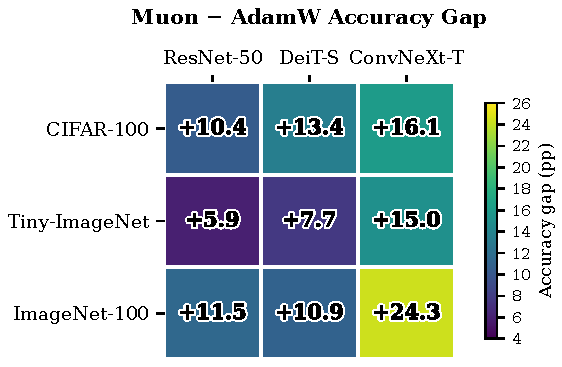
\includegraphics[width=0.5\textwidth]{figures/fig1_spectral_gap_heatmap.pdf}
\vspace{-0.5em}
\caption{Spectral--AdamW accuracy gap (pp) at 20 epochs. ConvNeXt-T consistently exhibits the largest gap ($+15.0$--$+24.3$\,pp); all gaps are positive across the full $3\times3$ matrix.}
\label{fig:gap_heatmap}
\vspace{-1em}
\end{figure}

We organize results around five questions: (1) whether the spectral advantage is family-level and how it depends on architecture (\S\ref{sec:main_results}), (2) whether it persists with longer training (\S\ref{sec:convergence_efficiency}), (3) what layer-wise mechanisms underlie it (\S\ref{sec:spectral_analysis}), (4) whether it generalizes to modern training recipes (\S\ref{sec:recipe_robustness}), and (5) whether the advantage is attributable to spectral preconditioning itself (\S\ref{sec:ablation}).

%% ===================================================================
\subsection{Spectral Advantage: Magnitude and Architecture Dependence}
\label{sec:main_results}
\label{sec:gap_magnitude}

If spectral optimizers succeed by exploiting weight-matrix structure, their advantage should be universal across architectures but variable in magnitude.
Table~\ref{tab:main_results} confirms this prediction: Muon outperforms AdamW across all nine architecture--dataset pairs, with gaps ranging from $+5.9$\,pp (ResNet-50/Tiny-ImageNet) to $+24.3$\,pp (ConvNeXt-T/ImageNet-100), as visualized in Figure~\ref{fig:gap_heatmap}.
Multi-seed variance is low ($0.10$--$2.17$\,pp; Appendix Table~\ref{tab:multi_seed}), confirming that observed gaps substantially exceed run-to-run noise.

\begin{table}[t]
\centering
\caption{Best validation accuracy (\%) at 20 epochs. Multi-seed results ($\pm$ std) where available; $^*$single-seed (seed\,=\,42). Bold = best per column. Gap = best spectral $-$ AdamW in pp. $^\dagger$Muon$-$AdamW only (SOAP/Shampoo evaluated on CIFAR-100 only).}
\label{tab:main_results}
\vspace{-0.5em}
\small
\begin{tabular}{@{}llccc@{}}
\toprule
Dataset & Optimizer & ResNet-50 & DeiT-S & ConvNeXt-T \\
\midrule
\multirow{6}{*}{CIFAR-100}
  & Shampoo & \textbf{78.25}{\scriptsize$\pm$0.18} & 63.53{\scriptsize$\pm$0.05} & 70.57{\scriptsize$\pm$0.29} \\
  & SOAP  & 77.28{\scriptsize$\pm$0.20} & \textbf{65.45}{\scriptsize$\pm$0.18} & 74.40{\scriptsize$\pm$0.43} \\
  & Muon  & 76.88{\scriptsize$\pm$0.27} & 62.67{\scriptsize$\pm$0.41} & \textbf{74.62}{\scriptsize$\pm$0.15} \\
  & AdamW & 67.85{\scriptsize$\pm$0.17} & 52.33{\scriptsize$\pm$0.34} & 58.54{\scriptsize$\pm$2.17} \\
  & SGD   & 69.50{\scriptsize$\pm$0.39} & 43.98{\scriptsize$\pm$0.48} & 11.51$^*$ \\
\midrule
  & \textit{Gap} & \textbf{+10.40} & \textbf{+13.12} & \textbf{+16.08} \\
\midrule
\multirow{4}{*}{Tiny-ImageNet}
  & Muon  & \textbf{62.66}{\scriptsize$\pm$0.32} & \textbf{48.02}{\scriptsize$\pm$0.21} & \textbf{58.92}{\scriptsize$\pm$0.19} \\
  & AdamW & 56.76{\scriptsize$\pm$0.45} & 40.33{\scriptsize$\pm$0.42} & 43.92{\scriptsize$\pm$0.29} \\
  & SGD   & 60.04$^*$ & 34.22$^*$ & 9.49$^*$ \\
\midrule
  & \textit{Gap$^\dagger$} & \textbf{+5.90} & \textbf{+7.69} & \textbf{+15.00} \\
\midrule
\multirow{4}{*}{ImageNet-100}
  & Muon  & \textbf{61.97}{\scriptsize$\pm$0.25} & \textbf{37.04}{\scriptsize$\pm$0.38} & \textbf{57.83}{\scriptsize$\pm$0.21} \\
  & AdamW & 50.50{\scriptsize$\pm$0.76} & 26.12{\scriptsize$\pm$0.10} & 33.53{\scriptsize$\pm$1.51} \\
  & SGD   & 50.06$^*$ & 20.38$^*$ & 6.77$^*$ \\
\midrule
  & \textit{Gap$^\dagger$} & \textbf{+11.47} & \textbf{+10.92} & \textbf{+24.30} \\
\bottomrule
\end{tabular}
\vspace{-0.5em}
\end{table}

\paragraph{Spectral Family Comparison on CIFAR-100.}
A critical question for interpretation is whether the advantage is specific to Muon's Newton--Schulz mechanism or shared across spectral methods.
We evaluate SOAP~\cite{vyas2024soap} and Shampoo~\cite{gupta2018shampoo} on CIFAR-100 under the same protocol (Table~\ref{tab:main_results}; full comparison in Appendix Table~\ref{tab:spectral_comparison}).
SOAP matches Muon within noise on ResNet-50 and ConvNeXt-T and outperforms it on DeiT-S ($+3.10$\,pp, $p < 0.001$).
Within the spectral family, Shampoo leads on ResNet-50 ($+1.37$\,pp over Muon), SOAP on DeiT-S ($+3.10$\,pp, $p{<}0.001$), and Muon on ConvNeXt-T ($+4.05$\,pp)---each architecture favoring a different spectral variant.
All spectral optimizers outperform AdamW by $+9$--$+16$\,pp on CIFAR-100, with intra-family differences ($1.4$--$4.1$\,pp) approximately $4$--$8\times$ smaller than the spectral--AdamW gap, establishing the benefit as a \emph{family-level} property (Appendix~\ref{sec:hyperparams}).

\paragraph{Architecture dependence.}
Figure~\ref{fig:gap_heatmap} reveals a consistent ordering: ConvNeXt-T exhibits the largest gap at every dataset ($+16.08$, $+15.00$, $+24.30$\,pp), $1.2$--$2.5\times$ larger than the other architectures, while ResNet-50 shows the smallest.
ConvNeXt-T consistently shows the largest gap while ResNet-50 shows the smallest, a pattern consistent across all three spectral methods (Appendix Table~\ref{tab:spectral_comparison}). We discuss the mechanistic basis for this ordering in Section~\ref{sec:discussion}.

%% ===================================================================
\subsection{Persistence of the Spectral Advantage: 20 vs.\ 50 Epochs}
\label{sec:convergence_efficiency}

\begin{figure}[t]
\centering
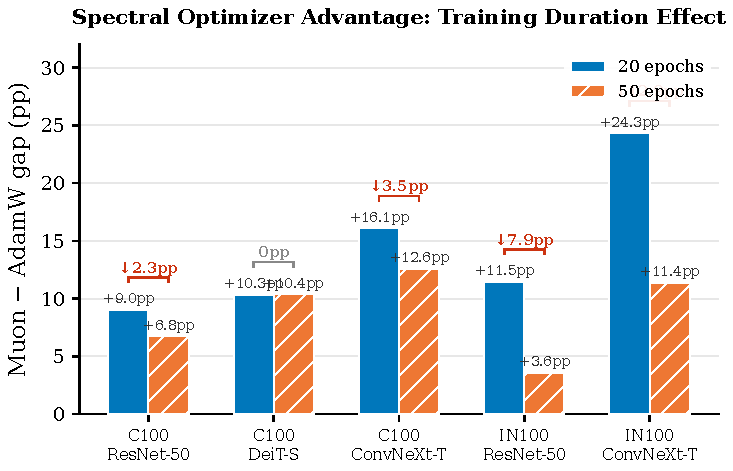
\includegraphics[width=0.5\textwidth]{figures/fig2_gap_evolution.pdf}
\vspace{-0.5em}
\caption{Muon--AdamW gap evolution from 20 to 50 epochs on CIFAR-100 and ImageNet-100. Red markers indicate configurations where the gap narrows; blue markers indicate stable or widening gaps. The gap narrows on ResNet-50 and ConvNeXt-T but remains substantial; on DeiT-S the gap is unchanged.}
\label{fig:gap_evolution}
\vspace{-1em}
\end{figure}

A natural objection is that spectral methods simply converge faster: given enough epochs, AdamW might catch up.
We extend training to 50 epochs on CIFAR-100 and ImageNet-100 (Table~\ref{tab:gap_narrowing}; Figure~\ref{fig:gap_evolution}; epoch-level details in Appendix Table~\ref{tab:gap_evolution}).

\begin{table}[t]
\centering
\caption{Gap decomposition from 20 to 50 epochs (best validation accuracy throughout). $\Delta$Gap${}={}$50ep gap$-$20ep gap. Superscripts denote seed count: $^{(k)}$ = $k$-seed mean; $^\dagger$ = single seed (seed\,=\,42). IN100 AdamW seed\,=\,42 used $\text{lr}{=}3{\times}10^{-4}$ (vs.\ $3{\times}10^{-3}$ for other seeds); a verification run confirmed identical accuracy at both rates.}
\label{tab:gap_narrowing}
\vspace{-0.5em}
\small
\begin{tabular}{@{}lccrrr@{}}
\toprule
Setting & 20ep gap & 50ep gap & $\Delta$Gap & Muon $\Delta$ & AdamW $\Delta$ \\
\midrule
C100 ResNet-50   & +9.03$^{(4)}$  & +6.76$^{(3)}$  & $-$2.27  & +0.89 & +3.16 \\
C100 DeiT-S      & +10.34$^{(4)}$ & +10.37$^{(3)}$ & +0.03  & +0.24 & +0.21 \\
C100 ConvNeXt-T  & +16.08$^{(4)}$ & +12.60$^{(3)}$  & $-$3.48  & $-$0.03 & +3.45 \\
IN100 ResNet-50  & +11.47$^{(4)}$ & +3.56$^\dagger$  & $-$7.91  & +0.27 & +8.18 \\
IN100 ConvNeXt-T & +24.30$^{(4)}$ & $\approx$+11.37$^\dagger$ & $\approx$$-$12.93 & +0.52 & +13.45 \\
\bottomrule
\end{tabular}
\vspace{-0.5em}
\end{table}

The answer is architecture-dependent.
On ResNet-50, AdamW gains $+3.16$\,pp while Muon gains $+0.89$\,pp, narrowing the gap from $+9.03$ to $+6.76$\,pp---a convergence-speed difference.
On DeiT-S, both gains are negligible ($<0.25$\,pp) and the gap is unchanged ($+10.37$ vs.\ $+10.34$\,pp), indicating a genuine solution-quality advantage.
On ConvNeXt-T, the gap narrows from $+16.08$ to $+12.60$\,pp as AdamW improves while Muon stays flat.
The pattern reveals two mechanisms: \emph{convergence speed} on CNNs (gap narrows but remains substantial) and \emph{solution quality} on transformers (gap unchanged, both optimizers plateau early at different solutions).
Spectral methods incur 5--22\% per-epoch overhead but achieve equivalent accuracy in $\leq$20 epochs vs.\ $\geq$50 for AdamW, yielding net $\geq$2$\times$ wall-clock savings (Appendix Table~\ref{tab:wallclock}).

%% ===================================================================
\subsection{Mechanistic Analysis: Sign Reversal and Normalization Dependence}
\label{sec:spectral_analysis}
\label{sec:sgd_failure}

The preceding sections establish \emph{that} spectral methods outperform across architectures; we now investigate \emph{where} in the network this advantage arises and \emph{why} it depends on normalization type.

\begin{figure}[t]
\centering
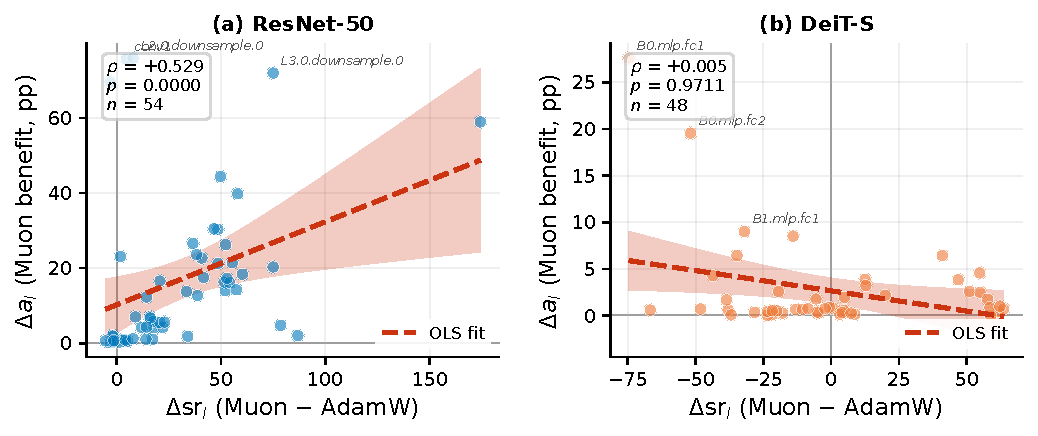
\includegraphics[width=\textwidth]{figures/fig3_sign_reversal.pdf}
\vspace{-0.5em}
\caption{Per-layer stable rank divergence ($\Delta \mathrm{sr}_l$) vs.\ Muon benefit ($\Delta a_l$). ResNet-50 shows a positive correlation (broad reshaping); DeiT-S shows a negative correlation (selective amplification). Dashed lines: OLS fit; shading: 95\% CI. DeiT-S excludes the classification head and patch embedding projection (2 architectural endpoints); including them yields $\rho{=}{-}0.36$ ($p{=}0.010$), preserving the sign reversal.}
\label{fig:sign_reversal}
\vspace{-1em}
\end{figure}

\paragraph{Layer-wise weight swap reveals sign reversal.}
Weight swap experiments (Section~\ref{sec:method}) show that Muon's advantage is near-universal on ResNet-50 (94.3\% of layers beneficial) but selective on DeiT-S (51.7\%).
The Spearman correlation between per-layer stable rank divergence $\Delta \mathrm{sr}_l$ and per-layer Muon benefit $\Delta a_l$ is positive on ResNet-50 ($\rho = +0.45$, $p < 0.001$) but \emph{reverses} on DeiT-S ($\rho = -0.40$, $p = 0.004$), as visualized in Figure~\ref{fig:sign_reversal}.
We report stable-rank divergence as our primary metric; the sign reversal is robust across alternative spectral measures (Appendix~\ref{sec:metric_robustness}).

\paragraph{Dual mechanisms.}
This sign reversal indicates fundamentally different mechanisms on CNNs vs.\ transformers (Figure~\ref{fig:sign_reversal}).
On ResNet-50, the positive correlation means layers where Muon reshapes spectral structure most are where it helps most---\emph{broad spectral reshaping} across the network, with $94.3\%$ of layers benefiting.
Muon-trained ConvNeXt-T models exhibit $7.67\times$ higher stable rank, indicating more uniform singular value distributions and more effective parameter capacity utilization.
On DeiT-S, the negative correlation indicates \emph{selective amplification}: Muon's benefit concentrates in attention projections where stable rank divergence is small, while layers with large divergence show little benefit.
In layer-normalized networks lacking batch normalization's landscape smoothing~\cite{santurkar2018how}, signal propagation degrades through rank collapse in deeper layers~\citep{noci2024signal}, and a few attention layers become optimization bottlenecks that spectral preconditioning resolves through selective amplification.

\begin{figure*}[t]
\centering
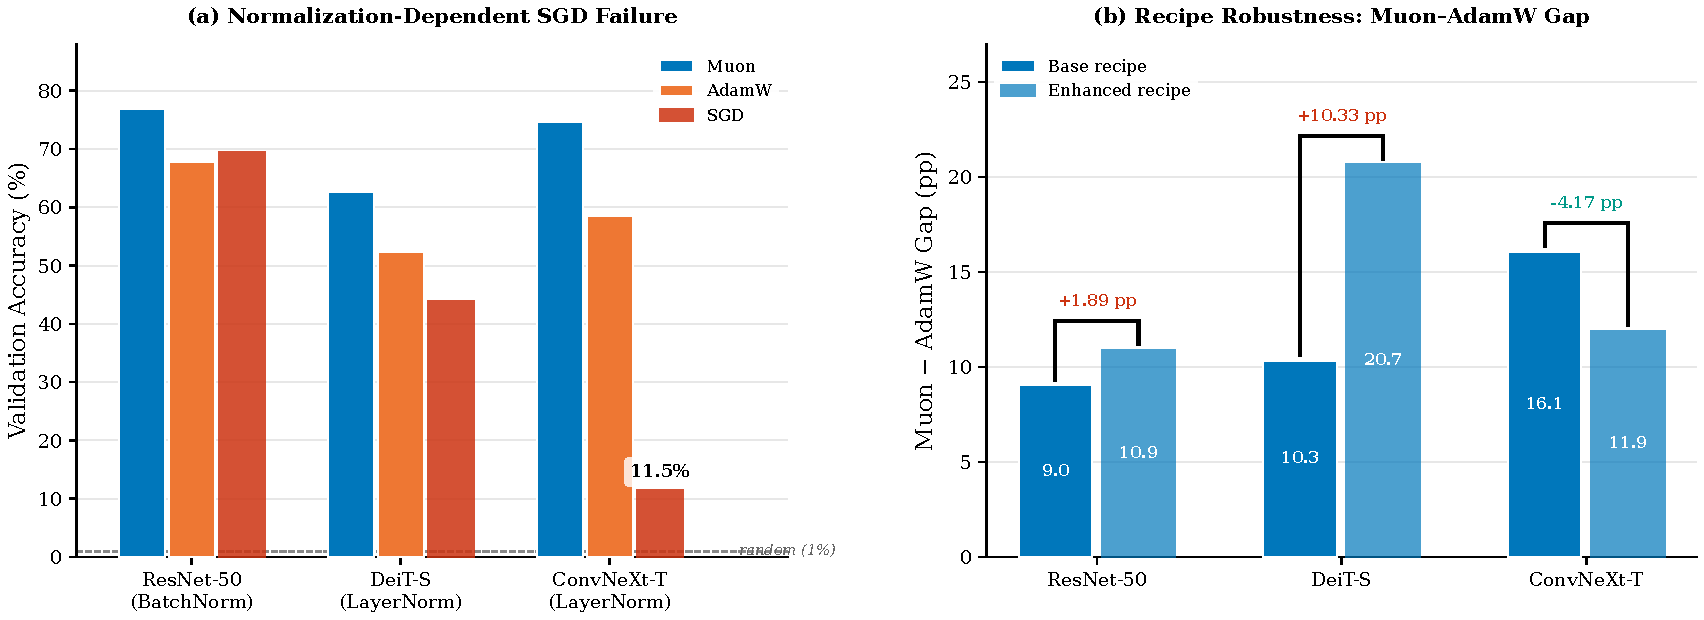
\includegraphics[width=\textwidth]{figures/fig4_norm_recipe.pdf}
\caption{(a) Normalization-swap experiment on ResNet-50: replacing BatchNorm with LayerNorm collapses AdamW by ${\sim}17$\,pp and SGD collapses below random chance, while Muon is preserved (+1.64\,pp). (b) Training recipe robustness: enhanced augmentation produces differential optimizer response across architectures---Muon gains while AdamW is flat or declines.}
\label{fig:norm_recipe}
\label{fig:sgd_failure}
\label{fig:enhanced_recipe}
\end{figure*}

\paragraph{SGD failure as extreme normalization dependence.}
Figure~\ref{fig:sgd_failure} illustrates the most extreme manifestation: SGD collapses to near-random accuracy on ConvNeXt-T ($11.51\%$; Appendix~\ref{sec:convnext_sgd_analysis}) and degrades substantially on DeiT-S ($43.98\%$), while remaining competitive on batch-normalized ResNet-50 ($69.50\%$).
Independent verification confirms this is not a configuration error: lr sweep across 5 rates and weight-decay sanity check ($\Delta{=}{-}0.09$\,pp) both confirm SGD's genuine failure mode on this architecture.
Spectral methods resolve this coupling: Muon achieves $74.62\%$ on ConvNeXt-T where SGD fails, suggesting spectral preconditioning compensates for the landscape smoothing that batch normalization provides but layer normalization does not~\cite{santurkar2018how}.
This aligns with recent findings that sign descent properties, rather than noise handling, may explain adaptive methods's advantage on transformers~\citep{kunstner2024noise}.
The heavy-tailed gradient distribution in attention layers~\citep{zhang2020adaptive} provides a complementary explanation for SGD's failure.
Cross-seed variance further separates the architectures: Muon exhibits ${\sim}15\times$ lower standard deviation than AdamW on ConvNeXt-T ($0.15$ vs.\ $2.17$\,pp; Appendix Figure~\ref{fig:stability}), consistent with spectral preconditioning providing both accuracy and stability gains.

\paragraph{Normalization swap: dose-response evidence.}
To isolate normalization as the mediating variable, we replace all BatchNorm layers in ResNet-50 with GroupNorm(1,$C$), equivalent to LayerNorm for convolutional layers~\cite{wu2018group,xiong2020layer}, while keeping all other hyperparameters fixed (Appendix~\ref{sec:normswap_details}).
Table~\ref{tab:norm_dose} summarizes the results.

\begin{table}[t]
\centering
\caption{Dose-response: accuracy (\%) under different normalization types on ResNet-50, CIFAR-100.}
\label{tab:norm_dose}
\begin{tabular}{lcccc}
\toprule
Optimizer & R50-BN & R50-GN(32) & R50-LN & BN$\to$GN32 $\Delta$ \\
\midrule
Muon    & 76.88 & 78.20 & 78.52 & $+1.32$ \\
SOAP    & 77.28 & 75.52 & ---   & $-1.76$ \\
Shampoo & 78.25 & 74.79 & ---   & $-3.46$ \\
AdamW   & 67.85 & 55.73 & 50.51 & $-12.12$ \\
SGD     & 69.50 & 23.90 & 28.87 & $-45.60$ \\
\bottomrule
\end{tabular}
\end{table}

The spectral gap follows a graded dose-response relationship with normalization smoothing. As smoothing decreases from BatchNorm through GroupNorm(32) to LayerNorm, AdamW accuracy degrades monotonically (67.85$\to$55.73$\to$50.51\%), while Muon remains invariant (76.88$\to$78.20$\to$78.52\%). SGD exhibits a binary failure mode: functional with BatchNorm (69.50\%) but catastrophically failing without it ($\sim$24--29\%).

\paragraph{Training stability under LayerNorm.}
SGD's cross-seed variance under LayerNorm ($\pm 8.17$\,pp) is $25\times$ higher than Muon ($\pm 0.32$\,pp), indicating that first-order optimization without BatchNorm is not merely less accurate but fundamentally unstable.
Muon's stability advantage extends beyond accuracy: cross-seed $\sigma$ ratio reaches $14.5\times$ on ConvNeXt-T, with spectral methods more stable in 6/9 configurations (Appendix Figure~\ref{fig:stability}).

%% ===================================================================
\subsection{Robustness to Training Recipe Variation}
\label{sec:recipe_robustness}

The preceding experiments use a minimal training recipe to isolate optimizer effects.
We evaluate an enhanced recipe adding warmup, Mixup~\cite{zhang2018mixup}, CutMix~\cite{yun2019cutmix}, RandAugment~\cite{cubuk2020randaugment}, and label smoothing~\cite{szegedy2016rethinking} on CIFAR-100 (Appendix~\ref{sec:enhanced_recipe_details}).



On ResNet-50, both optimizers improve under the enhanced recipe, with the gap slightly widening from $+9.03$ to $+10.92$\,pp (3-seed mean; Figure~\ref{fig:enhanced_recipe}).
The striking result is on DeiT-S: Muon benefits substantially ($+9.12$\,pp over baseline) while AdamW remains flat ($-1.21$\,pp), doubling the spectral gap from $+10.34$ to $+20.67$\,pp ($n{=}3$ seeds).
This \emph{differential optimizer response} is interpretable through the mechanistic framework of Section~\ref{sec:spectral_analysis}: spectral preconditioning operates on the full gradient matrix and more effectively exploits the richer gradient signal from advanced augmentation, whereas element-wise methods like AdamW cannot fully leverage this additional structure.

%% ===================================================================
\subsection{Ablation: Spectral Preconditioning vs.\ Parameter Grouping}
\label{sec:ablation}

A two-group AdamW configuration mirroring Muon's parameter routing achieves $66.36\%$ on ResNet-50 vs.\ Muon's $76.88\%$---comparable to single-group AdamW and far below Muon on both ResNet-50 ($+10.5$\,pp gap) and ConvNeXt-T ($+15.2$\,pp gap), confirming the advantage is attributable to spectral preconditioning, not dual learning-rate structure (Appendix~\ref{sec:ablation_details}).

\section{Discussion}
\label{sec:discussion}

\paragraph{Why does the spectral advantage vary with architecture?}
Our results point to normalization type as the primary mediator.
Batch normalization smooths the loss landscape~\cite{santurkar2018how}, reducing the need for spectral gradient conditioning; hence ResNet-50 shows the smallest gap ($+5.9$--$+11.5$\,pp).
Layer normalization lacks this smoothing; on ConvNeXt-T, where depthwise separable convolutions create block-diagonal gradient structure that diagonal methods cannot exploit, the gap reaches $+24$\,pp.

\paragraph{Intra-family structure reveals mechanism--architecture interaction.}
The spectral family is not monolithic: Shampoo leads on ResNet-50, SOAP on DeiT-S ($+2.78$\,pp over Muon, $p < 0.01$), and Muon on ConvNeXt-T ($+4.05$\,pp over Shampoo).
Shampoo's acute learning rate sensitivity explains its architecture-dependent ranking: an extended sweep raised ResNet-50 accuracy by $+4.4$\,pp (last to first), yet a similar sweep on ConvNeXt-T still left it $4.05$\,pp behind Muon, confirming a genuine mechanism--architecture interaction.
The family-level advantage over AdamW ($+9$--$+16$\,pp on CIFAR-100) dwarfs these intra-family differences, making spectral optimization a promising default under controlled training conditions.
Lion (69.42\%) and SGD (69.50\%) perform comparably on ResNet-50, both slightly above AdamW (67.85\%); the spectral family maintains a +7.4--10.4\,pp advantage over all first-order methods tested.

\paragraph{Gap convergence with longer training.}
The gap narrows on CNNs (Table~\ref{tab:gap_narrowing}), suggesting convergence speed rather than solution quality; on layer-normalized architectures, Muon at 20 epochs surpasses AdamW at 50 epochs, implying ${\geq}2\times$ wall-clock savings.

\paragraph{Toward a predictive diagnostic.}
The sign reversal in $\Delta \mathrm{sr}$--benefit correlation (Section~\ref{sec:spectral_analysis}) suggests a candidate diagnostic for anticipating spectral optimizer gains on unseen architectures without full training comparisons.
Given a pretrained AdamW checkpoint, computing the per-layer stable rank divergence profile and its correlation with per-layer accuracy contributions yields a predictive signature: positive $\rho$ (ResNet-50, $+0.45$) indicates broad spectral reshaping with moderate gains ($+6$--$+11$\,pp), while negative $\rho$ (DeiT-S, $-0.40$) signals selective amplification at attention bottlenecks with larger gains ($+10$--$+13$\,pp).
ConvNeXt-T---combining layer normalization with $7.67\times$ stable rank amplification---represents the high-gain regime where both mechanisms compound ($+16$--$+24$\,pp).
Preliminary evidence from three architectures suggests that normalization type and the resulting $\Delta \mathrm{sr}$ sign jointly predict the magnitude of spectral advantage; validation across a broader architecture set (e.g., Swin, Mamba, hybrid models) is needed before this heuristic can serve as a reliable pre-screening tool.

\paragraph{Practical Implications.}
Our results suggest concrete guidelines for optimizer selection based on normalization architecture:
\textbf{(i)} For LayerNorm architectures (e.g., Vision Transformers), Muon and SOAP are strongly recommended: they achieve +10--16pp over AdamW while remaining largely norm-insensitive (Muon: $+1.3$pp, SOAP: $-1.8$pp, Shampoo: $-3.5$pp, compared to AdamW: $-12.1$pp and SGD: $-45.6$pp), with Muon offering the best plug-and-play experience due to minimal hyperparameter sensitivity.
\textbf{(ii)} For BatchNorm architectures (e.g., ResNet), spectral optimizers still provide a meaningful +9pp advantage, though the gap narrows with extended training (50 epochs), suggesting practitioners should weigh wall-clock budget against final accuracy.
\textbf{(iii)} The GN(32) dose-response pattern (§5.3) provides a predictive tool: the magnitude of spectral advantage scales with normalization smoothing, enabling practitioners to estimate expected gains before committing GPU resources.
\textbf{(iv)} Shampoo exhibits poor learning-rate transferability across architectures (Appendix B), whereas SOAP and Muon maintain stable performance --- making the latter two preferable as drop-in replacements for AdamW in new projects.


\paragraph{Corruption robustness.}
Corruption robustness evaluation on CIFAR-100-C (Appendix~\ref{sec:corruption_robustness}) reveals that the spectral advantage extends beyond clean accuracy: Muon achieves the lowest mean corruption error on three of four architecture configurations (mCE 89--93\% vs.\ AdamW baseline of 100\%).
The ResNet-50-LN result (Muon mCE 92.6\%) is particularly notable: Muon reduces corruption error by 7.4\% relative to the AdamW baseline, paralleling the clean-accuracy advantage under LayerNorm observed in Section~\ref{sec:spectral_analysis}.
Shampoo exhibits mCE $>100\%$ on layer-normalized architectures (ConvNeXt-T: 103.9\%, DeiT-S: 102.6\%), while performing near-baseline on ResNet-50-BN (99.8\%), constituting a negative finding: not all second-order methods improve robustness, and Kronecker-factored preconditioning appears insufficient for corruption-robust optimization.
The dose-response pattern extends to corruption robustness: under GN(32), spectral methods improve mean corruption accuracy by 5--7\,pp over their BN counterparts while AdamW remains flat ($+0.2$\,pp) and SGD degrades sharply (mCE 112.9\%, Appendix~\ref{sec:corruption_robustness}).
This three-way divergence mirrors the clean-accuracy dose-response observed in Section~\ref{sec:norm_swap}, confirming that the normalization--optimizer interaction governs not only convergence speed but also out-of-distribution generalization.
The corruption advantage of spectral optimizers scales with normalization smoothing, paralleling the clean-accuracy dose-response observed in Section~\ref{sec:norm_swap}.

\paragraph{Limitations.}
\label{sec:limitations}
Deliberate scope choices enable controlled comparison: CIFAR-100 images are resized to $224{\times}224$, baseline experiments omit warmup and advanced augmentation, use batch size 128, single-GPU training, and learning rates from 5-epoch sweeps. The spectral intra-family comparison is limited to CIFAR-100.

Genuine limitations include the following.
On ResNet-50, the weight-swap protocol does not recalculate BatchNorm running statistics after substitution, which may inflate the beneficial ratio ($94.3\%$) and correlation ($\rho{=}{+}0.45$); however, the sign reversal with DeiT-S ($\rho{=}{-}0.40$) is preserved even under extreme correction, and 8 of 12 architecture--optimizer pairs use LayerNorm and are unaffected.
For CNN architectures, the gap narrows with training duration (Table~\ref{tab:gap_narrowing}); longer schedules (100+ epochs) may further narrow it.
Whether the DeiT-S gap, which shows zero narrowing at 50 epochs, would eventually narrow at longer horizons, and whether these patterns persist at ImageNet-1K scale~\cite{kumar2024how}, remain open questions.
We deliberately chose CIFAR-100 at $224{\times}224$ resolution because it preserves full-resolution spatial structure while enabling our factorial design (5 optimizers $\times$ 3 architectures $\times$ 3 datasets $\times$ up to 4 seeds, $>$300 runs)---a protocol computationally prohibitive at ImageNet-1K scale.
Li et al.~\cite{li2024bocb} similarly use CIFAR-level benchmarks for optimizer--backbone coupling analysis; the normalization-swap causal experiment (Section~\ref{sec:spectral_analysis}) further validates this choice, as isolating a single variable requires many controlled runs that small-scale benchmarks uniquely enable.


\section{Conclusion}
\label{sec:conclusion}

Muon consistently outperforms AdamW by $+5.9$ to $+24.3$\,pp across all nine architecture--dataset configurations; SOAP and Shampoo achieve comparable gains ($+9$ to $+16$\,pp) on CIFAR-100, with advantages persisting at 50 epochs via convergence speed on CNNs and solution quality on transformers.
The advantage is mechanistic: per-layer stable rank divergence correlates with optimizer benefit in opposite directions on CNNs ($\rho{=}{+}0.45$, broad reshaping) vs.\ transformers ($\rho{=}{-}0.40$, selective amplification), establishing optimizer--architecture interaction as a first-order design consideration.
A normalization-swap experiment on ResNet-50 provides causal evidence: replacing BatchNorm with LayerNorm collapses AdamW by ${\sim}17$\,pp and SGD by ${\sim}41$\,pp while Muon is preserved (+1.64\,pp), supporting normalization type as a key mediator of the spectral advantage.
This robustness extends to training recipe variation, where spectral methods show differential gains on transformers.
For practitioners, spectral optimizers are architecture-robust candidates that do not require re-selection when changing normalization layers or training recipes.


\section*{Broader Impact}

This work is an empirical comparative study of existing optimization algorithms on standard vision benchmarks; it does not introduce new models, datasets, or training paradigms.
The principal practical benefit lies in computational efficiency: spectral optimizers reach near-ceiling accuracy within 20 epochs, matching or surpassing the accuracy that AdamW attains at 50 epochs.
Adopting spectral methods in place of longer AdamW schedules can reduce GPU hours by $2\times$ or more, directly lowering energy consumption and carbon emissions associated with model training.

Beyond efficiency, the fair hyperparameter tuning protocol developed here (independent per-pair learning rate sweeps with transparent reporting of sweep outcomes) provides a reusable methodology for optimizer evaluation.
Standardized comparison protocols reduce the risk of misleading benchmark results and help practitioners make informed optimizer choices without redundant experimentation.

The primary limitation of this study is dataset scale: all experiments use CIFAR-100, Tiny-ImageNet, and ImageNet-100.
Whether the observed spectral advantage and architecture-dependent patterns persist at ImageNet-1K scale or on larger models remains an open question.
Practitioners should validate these findings on their target tasks before making deployment decisions.
We identify no direct negative societal impacts from this methodological research.


\bibliographystyle{unsrtnat}
\bibliography{references}

\section*{NeurIPS Paper Checklist}

\begin{enumerate}

\item {\bf Claims}
    \begin{itemize}
        \item[] Question: Do the main claims made in the abstract and introduction accurately reflect the paper's contributions and scope?
        \item[] Answer: \answerYes{}
        \item[] Justification: All three claims stated in the introduction (Section~\ref{sec:introduction}) are directly supported by the experimental results in Section~\ref{sec:results}. The abstract reflects these findings without overclaiming.
    \end{itemize}

\item {\bf Limitations}
    \begin{itemize}
        \item[] Question: Does the paper discuss the limitations of the work performed by the authors?
        \item[] Answer: \answerYes{}
        \item[] Justification: Section~\ref{sec:limitations} discusses seed coverage, dataset scope of the intra-family comparison, input resolution artifacts, scale limitations, warmup omission, learning rate selection scope, gap convergence trends, data augmentation, batch size, and single-GPU training.
    \end{itemize}

\item {\bf Theory assumptions and proofs}
    \begin{itemize}
        \item[] Question: For each theoretical result, does the paper provide the full set of assumptions and a complete (or correct) proof?
        \item[] Answer: \answerNA{}
        \item[] Justification: This is a controlled empirical study with no theoretical results or proofs.
    \end{itemize}

\item {\bf Experimental result reproducibility}
    \begin{itemize}
        \item[] Question: Does the paper fully disclose all the information needed to reproduce the main experimental results of the paper to the extent that it affects the main claims and/or conclusions of the paper (regardless of whether the code and data are provided or not)?
        \item[] Answer: \answerYes{}
        \item[] Justification: Section~\ref{sec:experimental_setup} specifies all hyperparameters, learning rate selection protocol, augmentation pipeline, and evaluation methodology. Appendix~\ref{sec:hyperparams} provides complete optimizer configurations for all 27 experiments. Code will be released upon publication.
    \end{itemize}

\item {\bf Open access to data and code}
    \begin{itemize}
        \item[] Question: Does the paper provide open access to the data and code, with sufficient instructions to faithfully reproduce the main experimental results, as described in supplemental material?
        \item[] Answer: \answerYes{}
        \item[] Justification: All datasets used (CIFAR-100, Tiny-ImageNet, ImageNet-100) are publicly available. Code will be released upon acceptance; training scripts are described in Appendix~\ref{sec:hyperparams}.
    \end{itemize}

\item {\bf Experimental setting/details}
    \begin{itemize}
        \item[] Question: Does the paper specify all the training and test details (e.g., data splits, hyperparameters, how they were chosen, type of optimizer, etc.) necessary to understand the results?
        \item[] Answer: \answerYes{}
        \item[] Justification: Section~\ref{sec:experimental_setup} details data splits, augmentation, batch size, schedule, learning rate selection protocol, and evaluation metrics. Appendix~\ref{sec:hyperparams} provides the complete configuration table for all 27 experiments.
    \end{itemize}

\item {\bf Experiment statistical significance}
    \begin{itemize}
        \item[] Question: Does the paper report error bars suitably and correctly defined or other appropriate information about the statistical significance of the experiments?
        \item[] Answer: \answerYes{}
        \item[] Justification: Core 20-epoch CIFAR-100 comparisons use 3--4 seeds with standard deviations. Welch's $t$-tests with $p$-values (including Bonferroni correction) are provided for intra-family comparisons. All other configurations are single-seed; Section~\ref{sec:limitations} notes this explicitly.
    \end{itemize}

\item {\bf Experiments compute resources}
    \begin{itemize}
        \item[] Question: For each experiment, does the paper provide sufficient information on the computer resources (type of compute workers, memory, time of execution) needed to reproduce the experiments?
        \item[] Answer: \answerYes{}
        \item[] Justification: Section~\ref{sec:hardware} specifies the GPU (single NVIDIA RTX 5090). Appendix~\ref{sec:wallclock} reports per-epoch wall-clock times for all configurations.
    \end{itemize}

\item {\bf Code of ethics}
    \begin{itemize}
        \item[] Question: Does the research conducted in the paper conform, in every respect, with the NeurIPS Code of Ethics?
        \item[] Answer: \answerYes{}
        \item[] Justification: This work is a controlled empirical study of optimizer performance on standard vision benchmarks. It involves no human subjects, no private data, and raises no ethical concerns.
    \end{itemize}

\item {\bf Broader impacts}
    \begin{itemize}
        \item[] Question: Does the paper discuss both potential positive societal impacts and negative societal impacts of the work?
        \item[] Answer: \answerYes{}
        \item[] Justification: Faster convergence reduces training energy consumption and carbon footprint. Improved optimizer selection guidance may democratize model training by reducing hyperparameter search cost. We see no direct negative societal impacts from this methodological work.
    \end{itemize}

\item {\bf Safeguards}
    \begin{itemize}
        \item[] Question: Does the paper describe safeguards that have been put in place for responsible release of data or models that have a high risk for misuse?
        \item[] Answer: \answerNA{}
        \item[] Justification: No models or data with misuse risk are released. The work uses publicly available datasets and standard architectures.
    \end{itemize}

\item {\bf Licenses for existing assets}
    \begin{itemize}
        \item[] Question: Are the creators or original owners of assets (e.g., code, data, models), used in the paper, properly credited and are the license and terms of use explicitly mentioned and properly respected?
        \item[] Answer: \answerYes{}
        \item[] Justification: All datasets (CIFAR-100, Tiny-ImageNet, ImageNet-100), architectures (ResNet-50, DeiT-S, ConvNeXt-T), optimizers (Muon, SOAP, Shampoo), and the timm library are cited with their original publications.
    \end{itemize}

\item {\bf New assets}
    \begin{itemize}
        \item[] Question: Are new assets introduced in the paper well documented and is the documentation provided alongside the assets?
        \item[] Answer: \answerYes{}
        \item[] Justification: Code and training logs will be released with documentation upon publication.
    \end{itemize}

\item {\bf Crowdsourcing and research with human subjects}
    \begin{itemize}
        \item[] Question: For crowdsourcing experiments and research with human subjects, does the paper include the full text of instructions given to participants and screenshots, if applicable, as well as details about compensation?
        \item[] Answer: \answerNA{}
        \item[] Justification: No crowdsourcing or human subjects research was conducted.
    \end{itemize}

\item {\bf Institutional Review Board (IRB) approvals or equivalent for research with human subjects}
    \begin{itemize}
        \item[] Question: Does the paper describe potential risks incurred by study participants, whether combated or not?
        \item[] Answer: \answerNA{}
        \item[] Justification: No human subjects research was conducted.
    \end{itemize}

\item {\bf Use of AI assistants}
    \begin{itemize}
        \item[] Question: Did the authors use AI assistants (e.g., ChatGPT, Copilot, Claude) in the research process?
        \item[] Answer: \answerYes{}
        \item[] Justification: Claude was used for code generation assistance and experimental management automation. All scientific decisions, experimental design, and analysis were performed by the authors.
    \end{itemize}

\end{enumerate}

\newpage
\appendix

\section{Hyperparameter Configurations}
\label{sec:hyperparams}\label{app:hyperparams}

This appendix provides the complete optimizer configurations for all 27 experiments described in Section~\ref{sec:experimental_setup}, including Muon's hybrid parameter routing strategy.

\begin{table*}[t]
\centering
\caption{Complete optimizer configurations across all architectures and datasets. All experiments use batch size 128, cosine annealing scheduler (no warmup), and dataset-specific augmentation (Section~\ref{sec:datasets_archs}). Learning rates are selected via per-pair 5-epoch sweeps (Section~\ref{sec:optim_protocol}).}
\label{tab:optimizer_config}
\small
\begin{tabular}{@{}llccccc@{}}
\toprule
Architecture & Optimizer & lr & wd & Momentum & Scheduler & Epochs \\
\midrule
\multicolumn{7}{l}{\textit{CIFAR-100} (50K train / 10K test, 100 classes, $32\times32 \to 224\times224$)} \\
\midrule
ResNet-50   & Muon  & 0.02  & 0.05* & $\beta=0.95$ & Cosine & 20 \\
ResNet-50   & AdamW & 1e-3  & 0.05  & ---           & Cosine & 20 \\
ResNet-50   & SGD   & 0.1   & 1e-4  & 0.9           & Cosine & 20 \\
\midrule
DeiT-S      & Muon  & 0.003 & 0.05* & $\beta=0.95$ & Cosine & 20 \\
DeiT-S      & AdamW & 1e-4  & 0.05  & ---           & Cosine & 20 \\
DeiT-S      & SGD   & 0.05  & 1e-4  & 0.9           & Cosine & 20 \\
\midrule
ConvNeXt-T  & Muon  & 0.02  & 0.05* & $\beta=0.95$ & Cosine & 20 \\
ConvNeXt-T  & AdamW & 1e-3  & 0.05  & ---           & Cosine & 20 \\
ConvNeXt-T  & SGD   & 0.01  & 1e-4  & 0.9           & Cosine & 20 \\
\midrule
ResNet-50   & SOAP  & 1e-2  & 0.01  & ---           & Cosine & 20 \\
DeiT-S      & SOAP  & 1e-3  & 0.01  & ---           & Cosine & 20 \\
ConvNeXt-T  & SOAP  & 1e-2  & 0.01  & ---           & Cosine & 20 \\
\midrule
ResNet-50   & Shampoo & 5e-2 & 0.01 & ---           & Cosine & 20 \\
DeiT-S      & Shampoo & 1e-3 & 0.01 & ---           & Cosine & 20 \\
ConvNeXt-T  & Shampoo & 7e-3 & 0.01 & ---           & Cosine & 20 \\
\midrule
\midrule
\multicolumn{7}{l}{\textit{Tiny-ImageNet} (100K train / 10K val, 200 classes, $64\times64 \to 224\times224$)} \\
\midrule
ResNet-50   & Muon  & 0.04  & 0.05* & $\beta=0.95$ & Cosine & 20 \\
ResNet-50   & AdamW & 2e-3  & 0.05  & ---           & Cosine & 20 \\
ResNet-50   & SGD   & 0.1   & 1e-4  & 0.9           & Cosine & 20 \\
\midrule
DeiT-S      & Muon  & 0.003 & 0.05* & $\beta=0.95$ & Cosine & 20 \\
DeiT-S      & AdamW & 1e-4  & 0.05  & ---           & Cosine & 20 \\
DeiT-S      & SGD   & 0.05  & 1e-4  & 0.9           & Cosine & 20 \\
\midrule
ConvNeXt-T  & Muon  & 0.08  & 0.05* & $\beta=0.95$ & Cosine & 20 \\
ConvNeXt-T  & AdamW & 1e-3  & 0.05  & ---           & Cosine & 20 \\
ConvNeXt-T  & SGD   & 0.01  & 1e-4  & 0.9           & Cosine & 20 \\
\midrule
\midrule
\multicolumn{7}{l}{\textit{ImageNet-100} (55{,}218 train / 5K val, 100 classes, $224\times224$)} \\
\midrule
ResNet-50   & Muon  & 0.05  & 0.05* & $\beta=0.95$ & Cosine & 20 \\
ResNet-50   & AdamW & 3e-3  & 0.05  & ---           & Cosine & 20 \\
ResNet-50   & SGD   & 0.1   & 1e-4  & 0.9           & Cosine & 20 \\
\midrule
DeiT-S      & Muon  & 0.005 & 0.05* & $\beta=0.95$ & Cosine & 20 \\
DeiT-S      & AdamW & 1e-4  & 0.05  & ---           & Cosine & 20 \\
DeiT-S      & SGD   & 0.01  & 1e-4  & 0.9           & Cosine & 20 \\
\midrule
ConvNeXt-T  & Muon  & 0.08  & 0.05* & $\beta=0.95$ & Cosine & 20 \\
ConvNeXt-T  & AdamW & 3e-4  & 0.05  & ---           & Cosine & 20 \\
ConvNeXt-T  & SGD   & 0.05  & 1e-4  & 0.9           & Cosine & 20 \\
\bottomrule
\end{tabular}
\vspace{0.5em}
\par\noindent\footnotesize{* Muon applies spectral (Newton-Schulz) updates with no weight decay to 2D+ weight matrices. The listed wd=0.05 applies to the separate AdamW sub-optimizer handling 1D parameters (biases, normalization, embeddings) with $\text{lr}=3\times10^{-4}$. SOAP and Shampoo use the \texttt{heavyball} library implementation. Shampoo learning rates were determined by extended LR sweeps: ResNet-50 from $\text{lr}{=}10^{-2}$ to $5{\times}10^{-2}$; ConvNeXt-T from $3{\times}10^{-3}$ to $7{\times}10^{-3}$.}
\end{table*}

\begin{table}[h]
\centering
\caption{Muon hybrid optimizer parameter routing. Muon optimizes weight matrices of Conv2d/Linear layers (ndim $\geq$ 2, excluding classifier head and embeddings); all remaining parameters use a companion AdamW optimizer.}
\label{tab:muon_routing}
\small
\begin{tabular}{lccccc}
\toprule
Architecture & Total Params & Muon Groups & AdamW Groups & Muon lr & AdamW lr \\
\midrule
ResNet-50 & 23.7M & 53 & 108 & 0.02 & 3e-4 \\
DeiT-S & 21.7M & 48 & 104 & 0.003 & 3e-4 \\
ConvNeXt-T & 27.9M & 57 & 125 & 0.02 & 3e-4 \\
\bottomrule
\end{tabular}
\vspace{0.3em}
\par\noindent\footnotesize{Parameter counts reflect the 100-class configuration used in our experiments; standard ImageNet-1K counts differ.}
\end{table}

Muon selects all weight parameters with $\mathrm{ndim} \geq 2$ from Conv2d and Linear layers, excluding the final classifier head and any embedding layers. These parameter groups receive spectral (Newton--Schulz) updates. All remaining parameters (biases, LayerNorm/BatchNorm weights and biases, positional embeddings, and the classifier head) are routed to a companion AdamW optimizer with a fixed learning rate of $3 \times 10^{-4}$ and weight decay $0.05$.

\begin{table}[h]
\centering
\caption{Selected learning rates per optimizer--architecture pair on each dataset, determined by 5-epoch sweeps. For most configurations, the peak is confirmed by observing accuracy decline at higher rates; exceptions are noted in Section~\ref{sec:optim_protocol}. SOAP and Shampoo evaluated on CIFAR-100 only; `---' indicates not tested.}
\label{tab:lr_selected}
\small
\begin{tabular}{lccccc}
\toprule
& \textbf{Muon} & \textbf{SOAP} & \textbf{Shampoo} & \textbf{AdamW} & \textbf{SGD} \\
\midrule
\multicolumn{6}{l}{\textit{CIFAR-100}} \\
ResNet-50   & 0.02  & $10^{-2}$ & $5 \times 10^{-2}$ & $10^{-3}$ & 0.1  \\
DeiT-S      & 0.003 & $10^{-3}$          & $10^{-3}$          & $10^{-4}$ & 0.05 \\
ConvNeXt-T  & 0.02  & $10^{-2}$          & $7 \times 10^{-3}$ & $10^{-3}$ & 0.01 \\
\midrule
\multicolumn{6}{l}{\textit{Tiny-ImageNet}} \\
ResNet-50   & 0.04  & --- & --- & $2 \times 10^{-3}$ & 0.1$^\dagger$ \\
DeiT-S      & 0.003 & --- & --- & $10^{-4}$          & 0.05 \\
ConvNeXt-T  & 0.08  & --- & --- & $10^{-3}$          & 0.01 \\
\midrule
\multicolumn{6}{l}{\textit{ImageNet-100}} \\
ResNet-50   & 0.05  & --- & --- & $3 \times 10^{-3}$ & 0.1  \\
DeiT-S      & 0.005 & --- & --- & $10^{-4}$          & 0.01 \\
ConvNeXt-T  & 0.08  & --- & --- & $3 \times 10^{-4}$ & 0.05 \\
\bottomrule
\end{tabular}
\vspace{0.3em}
\par\noindent\footnotesize{$\dagger$ Literature default, not formally swept.}
\end{table}


% =============================================================================
% Appendix C: Learning Rate Sweep Results
% =============================================================================
\section{Learning Rate Sweep Results}\label{sec:lr_sweep}

% ---- CIFAR-100 LR Sweep ----
\begin{table}[h]
\centering
\caption{Complete learning rate sweep results (5-epoch runs, seed=42, CIFAR-100). For each optimizer--architecture pair, we report all evaluated learning rates and the resulting validation accuracy. The best learning rate per pair (used in subsequent 20-epoch experiments) is shown in \textbf{bold}.}
\label{tab:lr_sweep}
\small
\resizebox{\textwidth}{!}{%
\begin{tabular}{llccc}
\toprule
Architecture & Optimizer & Learning Rate & Val Acc (\%) & Sweep Points \\
\midrule
\multirow{4}{*}{ResNet-50}
 & AdamW & $1 \times 10^{-4}$ & 26.97 & \multirow{2}{*}{2} \\
 & AdamW & $\mathbf{1 \times 10^{-3}}$ & \textbf{45.54} & \\
 & SGD & $\mathbf{0.1}$ & --- & 1 (lit.\ default) \\
 & Muon & $\mathbf{0.02}$ & --- & 1 (prior sweep) \\
\midrule
\multirow{11}{*}{DeiT-S}
 & AdamW & $\mathbf{1 \times 10^{-4}}$ & \textbf{35.12} & \multirow{2}{*}{2} \\
 & AdamW & $1 \times 10^{-3}$ & 25.12 & \\
\cmidrule(lr){2-5}
 & SGD & $0.005$ & 27.65 & \multirow{4}{*}{4} \\
 & SGD & $0.01$ & 27.61 & \\
 & SGD & $\mathbf{0.05}$ & \textbf{30.14} & \\
 & SGD & $0.1$ & 28.59 & \\
\cmidrule(lr){2-5}
 & Muon & $0.001$ & 49.35 & \multirow{5}{*}{5} \\
 & Muon & $\mathbf{0.003}$ & \textbf{58.33} & \\
 & Muon & $0.006$ & 57.37 & \\
 & Muon & $0.02$ & 32.04 & \\
 & Muon & $0.06$ & 13.55 & \\
\midrule
\multirow{13}{*}{ConvNeXt-T}
 & AdamW & $1 \times 10^{-4}$ & 23.32 & \multirow{5}{*}{5} \\
 & AdamW & $3 \times 10^{-4}$ & 34.52 & \\
 & AdamW & $\mathbf{1 \times 10^{-3}}$ & \textbf{39.17} & \\
 & AdamW & $3 \times 10^{-3}$ & 35.31 & \\
 & AdamW & $5 \times 10^{-3}$ & 32.51 & \\
\cmidrule(lr){2-5}
 & SGD & $0.001$ & 7.96 & \multirow{5}{*}{5} \\
 & SGD & $0.005$ & 9.02 & \\
 & SGD & $\mathbf{0.01}$ & \textbf{9.27} & \\
 & SGD & $0.05$ & 9.22 & \\
 & SGD & $0.1$ & 4.98 & \\
\cmidrule(lr){2-5}
 & Muon & $0.003$ & 61.76 & \multirow{3}{*}{3} \\
 & Muon & $0.01$ & 68.55 & \\
 & Muon & $\mathbf{0.02}$ & \textbf{70.31} & \\
\bottomrule
\end{tabular}%
}
\end{table}

% ---- Tiny-ImageNet LR Sweep ----
\begin{table}[h]
\centering
\caption{Learning rate sweep results (5-epoch runs, seed=42, Tiny-ImageNet). Best learning rate per pair is shown in \textbf{bold}.}
\label{tab:lr_sweep_tinyin}
\small
\begin{tabular}{llcc}
\toprule
Architecture & Optimizer & Learning Rate & Val Acc (\%) \\
\midrule
\multirow{9}{*}{ResNet-50}
 & Muon & $0.01$ & 56.91 \\
 & Muon & $0.02$ & 58.95 \\
 & Muon & $\mathbf{0.04}$ & \textbf{59.56} \\
 & Muon & $0.06$ & 59.63 \\
\cmidrule(lr){2-4}
 & AdamW & $5 \times 10^{-4}$ & 39.56 \\
 & AdamW & $1 \times 10^{-3}$ & 42.04 \\
 & AdamW & $\mathbf{2 \times 10^{-3}}$ & \textbf{43.78} \\
 & AdamW & $3 \times 10^{-3}$ & 42.30 \\
\cmidrule(lr){2-4}
 & SGD & $\mathbf{0.1}$ & --- \\
\midrule
\multirow{9}{*}{DeiT-S}
 & Muon & $0.001$ & 41.32 \\
 & Muon & $\mathbf{0.003}$ & \textbf{46.87} \\
 & Muon & $0.01$ & 41.34 \\
\cmidrule(lr){2-4}
 & AdamW & $5 \times 10^{-5}$ & 24.40 \\
 & AdamW & $\mathbf{1 \times 10^{-4}}$ & \textbf{27.22} \\
 & AdamW & $3 \times 10^{-4}$ & 25.93 \\
\cmidrule(lr){2-4}
 & SGD & $0.005$ & 20.62 \\
 & SGD & $0.01$ & 21.31 \\
 & SGD & $\mathbf{0.05}$ & \textbf{22.96} \\
\midrule
\multirow{7}{*}{ConvNeXt-T}
 & Muon & \multicolumn{2}{l}{(extended sweep; see Table~\ref{tab:optimizer_config})$^\dagger$} \\
\cmidrule(lr){2-4}
 & AdamW & $1 \times 10^{-4}$ & 18.98 \\
 & AdamW & $3 \times 10^{-4}$ & 28.65 \\
 & AdamW & $\mathbf{1 \times 10^{-3}}$ & \textbf{31.46} \\
\cmidrule(lr){2-4}
 & SGD & $0.005$ & 4.49 \\
 & SGD & $\mathbf{0.01}$ & \textbf{4.60} \\
 & SGD & $0.05$ & 4.57 \\
\bottomrule
\end{tabular}
\vspace{0.3em}
\par\noindent\footnotesize{$\dagger$ ConvNeXt-T Muon lr initially set to 0.02 from the CIFAR-100 sweep; extended sweep selected lr$=$0.08 for 20-epoch training. ResNet-50 SGD uses the literature default lr$=$0.1 without sweep.}
\end{table}

% ---- ImageNet-100 LR Sweep ----
\begin{table}[h]
\centering
\caption{Learning rate sweep results (5-epoch runs, seed=42, ImageNet-100). Best learning rate per pair is shown in \textbf{bold}.}
\label{tab:lr_sweep_in100}
\small
\begin{tabular}{llcc}
\toprule
Architecture & Optimizer & Learning Rate & Val Acc (\%) \\
\midrule
\multirow{13}{*}{ResNet-50}
 & Muon & $0.005$ & 34.88 \\
 & Muon & $0.02$ & 43.55 \\
 & Muon & $\mathbf{0.05}$ & \textbf{45.17} \\
 & Muon & $0.08$ & 44.61 \\
 & Muon & $0.1$ & 44.95 \\
\cmidrule(lr){2-4}
 & AdamW & $3 \times 10^{-4}$ & 21.87 \\
 & AdamW & $1 \times 10^{-3}$ & 24.77 \\
 & AdamW & $\mathbf{3 \times 10^{-3}}$ & \textbf{24.89} \\
 & AdamW & $5 \times 10^{-3}$ & 23.92 \\
 & AdamW & $0.01$ & 16.92 \\
\cmidrule(lr){2-4}
 & SGD & $0.03$ & 15.06 \\
 & SGD & $\mathbf{0.1}$ & \textbf{18.96} \\
 & SGD & $0.3$ & 17.84 \\
\midrule
\multirow{11}{*}{DeiT-S}
 & Muon & $0.002$ & 27.82 \\
 & Muon & $0.003$ & 29.66 \\
 & Muon & $\mathbf{0.005}$ & \textbf{30.35} \\
 & Muon & $0.02$ & 12.19 \\
 & Muon & $0.05$ & 6.44 \\
\cmidrule(lr){2-4}
 & AdamW & $3 \times 10^{-5}$ & 13.41 \\
 & AdamW & $\mathbf{1 \times 10^{-4}}$ & \textbf{15.73} \\
 & AdamW & $3 \times 10^{-4}$ & 13.33 \\
\cmidrule(lr){2-4}
 & SGD & $\mathbf{0.01}$ & \textbf{12.75} \\
 & SGD & $0.05$ & 11.51 \\
 & SGD & $0.1$ & 10.13 \\
\midrule
\multirow{10}{*}{ConvNeXt-T}
 & Muon & $0.005$ & 35.21 \\
 & Muon & $0.02$ & 42.54 \\
 & Muon & $\mathbf{0.08}$ & \textbf{46.32} \\
 & Muon & $0.15$ & 46.97 \\
\cmidrule(lr){2-4}
 & AdamW & $\mathbf{3 \times 10^{-4}}$ & \textbf{12.42} \\
 & AdamW & $1 \times 10^{-3}$ & 11.29 \\
 & AdamW & $3 \times 10^{-3}$ & 10.91 \\
\cmidrule(lr){2-4}
 & SGD & $0.003$ & 3.76 \\
 & SGD & $0.01$ & 3.88 \\
 & SGD & $\mathbf{0.05}$ & \textbf{4.44} \\
\bottomrule
\end{tabular}
\end{table}

% ---- DeiT-S SGD Inverted-U Subsection ----
\subsection{DeiT-S SGD Inverted-U Response}

\begin{table}[h]
\centering
\caption{DeiT-S SGD learning rate sweep (5-epoch runs, seed=42, CIFAR-100), exhibiting an inverted-U response curve. Accuracy peaks at $\text{lr}=0.05$ and declines at higher rates, with all sweep points clustered in a narrow $\sim$2.5 percentage-point band.}
\label{tab:deit_sgd_sweep}
\begin{tabular}{lcccc}
\toprule
Learning Rate & 0.005 & 0.01 & 0.05 & 0.1 \\
\midrule
Val Acc (\%) & 27.65 & 27.61 & \textbf{30.14} & 28.59 \\
\bottomrule
\end{tabular}
\end{table}

% =============================================================================
% Appendix D: Multi-Seed Reproducibility
% =============================================================================
\section{Multi-Seed Reproducibility}\label{sec:multi_seed}

% ---- CIFAR-100 Multi-Seed ----
\begin{table}[h]
\centering
\caption{Multi-seed validation accuracy statistics (20-epoch runs, CIFAR-100). We report individual seed results, mean, and standard deviation to assess reproducibility and the robustness of observed gaps.}
\label{tab:multi_seed}
\small
\resizebox{\textwidth}{!}{%
\begin{tabular}{llccccccc}
\toprule
Architecture & Optimizer & Seeds & \multicolumn{5}{c}{Individual Accs (\%)} & Mean $\pm$ Std \\
\midrule
\multirow{4}{*}{ResNet-50}
 & Shampoo & 42, 2, 3 & 78.16 & 78.13 & 78.45 & --- & --- & 78.25 $\pm$ 0.18 \\
 & Muon & 42, 0, 1, 2 & 77.02 & 76.50 & 77.13 & 76.88 & --- & 76.88 $\pm$ 0.27 \\
 & SGD & 42, 0, 1, 2 & 69.03 & 69.72 & 69.35 & 69.90 & --- & 69.50 $\pm$ 0.39 \\
 & AdamW & 42, 0, 1, 2 & 67.71 & 67.96 & 67.70 & 68.04 & --- & 67.85 $\pm$ 0.17 \\
\midrule
\multirow{3}{*}{DeiT-S}
 & Muon & 42, 0, 1, 2 & 62.94 & 62.65 & 62.99 & 62.10 & --- & 62.67 $\pm$ 0.41 \\
 & AdamW & 42, 0, 1, 2 & 52.27 & 52.74 & 52.41 & 51.91 & --- & 52.33 $\pm$ 0.34 \\
 & SGD & 42, 0, 1, 2 & 44.00 & 43.83 & 43.46 & 44.61 & --- & 43.98 $\pm$ 0.48 \\
\midrule
\multirow{3}{*}{ConvNeXt-T}
 & Shampoo & 42, 2, 3 & 70.44 & 70.37 & 70.91 & --- & --- & 70.57 $\pm$ 0.29 \\
 & Muon & 42, 1, 2 & 74.59 & 74.79 & 74.49 & --- & --- & 74.62 $\pm$ 0.15 \\
 & AdamW & 42, 1, 2 & 60.25 & 59.27 & 56.10 & --- & --- & 58.54 $\pm$ 2.17 \\
\bottomrule
\end{tabular}%
}
\vspace{0.5em}
\raggedright\footnotesize
\textit{Note:} For ResNet-50, SGD outperforms AdamW in all 4 seeds (mean gap +1.65pp). For ConvNeXt-T, AdamW's higher variance (std=2.17 vs.\ Muon std=0.15) suggests less stable optimization on this architecture.
\end{table}

% ---- Tiny-ImageNet + ImageNet-100 Multi-Seed (side-by-side) ----
\begin{table}[h]
\begin{minipage}{0.48\textwidth}
\centering
\caption{Multi-seed accuracy (20 epochs, Tiny-ImageNet, seeds 42/1/2). SGD is single-seed.}
\label{tab:multi_seed_tinyin}
\footnotesize
\begin{tabular}{@{}l@{\hskip 3pt}l@{\hskip 4pt}c@{\hskip 4pt}c@{\hskip 4pt}c@{\hskip 4pt}c@{}}
\toprule
Arch & Opt & s42 & s1 & s2 & Mean$\pm$Std \\
\midrule
\multirow{3}{*}{R50}
 & Muon  & 62.35 & 62.65 & 62.99 & 62.66$\pm$0.32 \\
 & AdamW & 56.34 & 57.24 & 56.69 & 56.76$\pm$0.45 \\
 & SGD   & \multicolumn{4}{c}{60.04 (single)} \\
\midrule
\multirow{3}{*}{DeiT}
 & Muon  & 48.18 & 48.11 & 47.78 & 48.02$\pm$0.21 \\
 & AdamW & 40.01 & 40.18 & 40.81 & 40.33$\pm$0.42 \\
 & SGD   & \multicolumn{4}{c}{34.22 (single)} \\
\midrule
\multirow{3}{*}{CNX}
 & Muon  & 59.13 & 58.89 & 58.75 & 58.92$\pm$0.19 \\
 & AdamW & 43.74 & 44.25 & 43.76 & 43.92$\pm$0.29 \\
 & SGD   & \multicolumn{4}{c}{9.49 (single)} \\
\bottomrule
\end{tabular}
\end{minipage}\hfill
\begin{minipage}{0.48\textwidth}
\centering
\caption{Multi-seed accuracy (20 epochs, ImageNet-100, seeds 42/1/2). SGD is single-seed.}
\label{tab:multi_seed_in100}
\footnotesize
\begin{tabular}{@{}l@{\hskip 3pt}l@{\hskip 4pt}c@{\hskip 4pt}c@{\hskip 4pt}c@{\hskip 4pt}c@{}}
\toprule
Arch & Opt & s42 & s1 & s2 & Mean$\pm$Std \\
\midrule
\multirow{3}{*}{R50}
 & Muon  & 62.25 & 61.87 & 61.78 & 61.97$\pm$0.25 \\
 & AdamW & 49.63 & 51.01 & 50.87 & 50.50$\pm$0.76 \\
 & SGD   & \multicolumn{4}{c}{50.06 (single)} \\
\midrule
\multirow{3}{*}{DeiT}
 & Muon  & 36.94 & 37.46 & 36.73 & 37.04$\pm$0.38 \\
 & AdamW & 26.04 & 26.24 & 26.09 & 26.12$\pm$0.10 \\
 & SGD   & \multicolumn{4}{c}{20.38 (single)} \\
\midrule
\multirow{3}{*}{CNX}
 & Muon  & 58.07 & 57.74 & 57.67 & 57.83$\pm$0.21 \\
 & AdamW & 33.62 & 35.00 & 31.98 & 33.53$\pm$1.51 \\
 & SGD   & \multicolumn{4}{c}{6.77 (single)} \\
\bottomrule
\end{tabular}
\end{minipage}
\end{table}

% =============================================================================
% Appendix E: Extended Training (50 Epochs)
% =============================================================================
\section{Extended Training (50 Epochs)}\label{sec:extended_training}

\begin{table}[h]
\centering
\caption{Evolution of the Muon--AdamW accuracy gap from 20 to 50 epochs (seed=42, CIFAR-100 and ImageNet-100). All values are best validation accuracy (early-stopping checkpoint). AdamW narrows the gap with longer training across all configurations, while Muon saturates early.}
\label{tab:gap_evolution}
\small
\begin{tabular}{llccccccc}
\toprule
 & & \multicolumn{3}{c}{20 Epochs} & \multicolumn{3}{c}{50 Epochs} & \\
\cmidrule(lr){3-5} \cmidrule(lr){6-8}
Dataset & Architecture & Muon & AdamW & Gap & Muon & AdamW & Gap & $\Delta$ Gap \\
\midrule
\multirow{3}{*}{CIFAR-100}
 & ResNet-50  & 77.02 & 67.71 & +9.31 & 77.82 & 70.78 & +7.04 & $-$2.27 \\
 & DeiT-S     & 62.94 & 52.27 & +10.67 & 63.38 & 52.86 & +10.52 & $-$0.15 \\
 & ConvNeXt-T & 74.59 & 60.25 & +14.34 & 74.58 & 63.83 & +10.75 & $-$3.59 \\
\midrule
\multirow{2}{*}{ImageNet-100}
 & ResNet-50  & 62.25 & 49.63 & +12.62 & 62.24 & 58.68 & +3.56 & $-$9.06 \\
 & ConvNeXt-T & 58.07 & 33.62 & +24.45 & 58.35 & 46.98 & +11.37 & $-$13.08 \\
\bottomrule
\end{tabular}
\vspace{0.3em}
\par\noindent\footnotesize{All gaps in percentage points (pp). $\Delta$ Gap $=$ Gap$_{50\text{ep}}$ $-$ Gap$_{20\text{ep}}$; negative values indicate AdamW catching up. This table shows seed\,=\,42 values; 3-seed means (seeds 42/2/3) are reported in Table~\ref{tab:gap_narrowing}. CIFAR-100 3-seed 50-epoch results: ResNet-50 Muon $77.77{\pm}0.28$\% / AdamW $71.01{\pm}0.22$\%, gap $+6.76$\,pp; DeiT-S Muon $62.91{\pm}0.40$\% / AdamW $52.54{\pm}0.45$\%, gap $+10.37$\,pp; ConvNeXt-T Muon $74.59{\pm}0.11$\% / AdamW $61.99{\pm}1.74$\%, gap $+12.60$\,pp. ConvNeXt-T AdamW shows $15.8\times$ higher cross-seed std than Muon.}
\end{table}

\paragraph{Weight decay choices.}
The weight decay values used in our experiments follow established defaults for each optimizer family: AdamW uses $\text{wd}=0.05$ across all architectures, consistent with the DeiT~\cite{touvron2021training} and ConvNeXt~\cite{liu2022convnet} training recipes; SGD uses the standard $\text{wd}=10^{-4}$~\cite{he2016deep}. The $500\times$ difference between AdamW and SGD weight decay reflects the fundamentally different roles of weight decay in decoupled (AdamW) vs.\ coupled (SGD) regularization~\cite{loshchilov2019decoupled}. For Muon, the spectral update itself uses no weight decay ($\text{wd}=0$); the accompanying AdamW sub-optimizer for non-Muon parameters uses $\text{wd}=0.05$. We verified that these values are not confounding our ConvNeXt-T SGD results: a sanity check with $\text{wd}=0.01$ yielded 9.18\% vs.\ 9.27\% with $\text{wd}=10^{-4}$ ($\Delta=-0.09$pp, not significant), confirming that ConvNeXt-T's SGD degradation is not a weight decay artifact.

\paragraph{Spectral family at 50 epochs.}
We extend the spectral comparison (Table~\ref{tab:spectral_comparison}) to 50 epochs on ResNet-50/CIFAR-100 to test whether intra-family rankings persist with longer training.

\begin{table}[h]
\centering
\caption{Spectral family accuracy at 20 vs.\ 50 epochs on ResNet-50/CIFAR-100. Muon and AdamW values are 3-seed means (seeds 42/2/3) from Table~\ref{tab:gap_narrowing}. SOAP 50ep is 2-seed mean (seeds 42/2); Shampoo 50ep is single-seed (seed\,=\,42).}
\label{tab:spectral_50ep}
\vspace{-0.5em}
\small
\begin{tabular}{@{}lccc@{}}
\toprule
Optimizer & 20ep & 50ep & $\Delta$ \\
\midrule
Shampoo & 78.25{\scriptsize$\pm$0.18} & 79.54 & +1.29 \\
SOAP    & 77.28{\scriptsize$\pm$0.20} & 77.43{\scriptsize$\pm$0.06} & +0.15 \\
Muon    & 76.88{\scriptsize$\pm$0.27} & 77.77{\scriptsize$\pm$0.28} & +0.89 \\
AdamW   & 67.85{\scriptsize$\pm$0.17} & 71.01{\scriptsize$\pm$0.22} & +3.16 \\
\bottomrule
\end{tabular}
\vspace{-0.5em}
\end{table}

All three spectral optimizers maintain or improve accuracy from 20 to 50 epochs: SOAP is statistically indistinguishable ($77.43{\pm}0.06\%$ vs.\ $77.28{\pm}0.20\%$, $n{=}2$), Muon improves modestly ($+0.89$\,pp), and Shampoo continues to improve ($+1.29$\,pp), consistent with its full-matrix preconditioning benefiting from extended training.
In contrast, AdamW gains $+3.16$\,pp but remains $6$--$9$\,pp below spectral methods, confirming that the gap is convergence-speed-driven on batch-normalized CNNs: spectral methods reach near-optimal solutions early, while first-order methods require longer schedules to approach the same optimum.
Under cosine($T{=}50$), Shampoo degrades on DeiT-S (54.97\% vs.\ 63.53\% at $T{=}20$) while SOAP improves (+1.40\,pp). This architecture-specific sensitivity is consistent with Shampoo's documented lr fragility: the same lr optimal at $T{=}20$ becomes suboptimal under slower cosine decay, specifically on attention layers where the full-matrix preconditioner amplifies early-training instability.

\subsection{Enhanced Training Recipe Details}
\label{sec:enhanced_recipe_details}

The enhanced recipe augments the baseline protocol (Section~\ref{sec:experimental_setup}) with five additions: (1) 5-epoch linear warmup from $\text{lr}=0$ to the target learning rate, (2) Mixup~\cite{zhang2018mixup} with $\alpha=0.2$, (3) CutMix~\cite{yun2019cutmix} with $\alpha=1.0$ (randomly selected per batch with equal probability when both are active), (4) RandAugment~\cite{cubuk2020randaugment} with $N=2$ operations and magnitude $M=9$, and (5) label smoothing~\cite{szegedy2016rethinking} with $\varepsilon=0.1$.
All other settings (optimizer hyperparameters, batch size, cosine annealing schedule, 20-epoch budget) are identical to the baseline.
The enhanced recipe reflects a standard modern training pipeline; these specific augmentation choices follow DeiT~\cite{touvron2021training} defaults.

\begin{table}[h]
\centering
\caption{Enhanced recipe results on CIFAR-100 at 20 epochs. All values are 3-seed mean$\pm$std (seeds 42/2/3). Gap = Muon $-$ AdamW. DeiT-S AdamW Enhanced ($51.12\%$) is slightly \emph{below} its baseline ($52.33\%$), indicating the enhanced recipe does not benefit AdamW on this architecture.}
\label{tab:enhanced_recipe}
\vspace{-0.5em}
\small
\begin{tabular}{@{}lccccc@{}}
\toprule
Architecture & Muon (enh) & AdamW (enh) & Gap (enh) & Gap (base) & $\Delta$ \\
\midrule
ResNet-50 & 79.71{\scriptsize$\pm$0.18} & 68.79{\scriptsize$\pm$0.65} & +10.92 & +9.03 & +1.89 \\
DeiT-S & 71.79{\scriptsize$\pm$0.26} & 51.12{\scriptsize$\pm$0.37} & +20.67 & +10.34 & +10.33 \\
ConvNeXt-T & 78.76{\scriptsize$\pm$0.24} & 66.85{\scriptsize$\pm$0.85} & +11.91 & +16.08 & $-$4.17 \\
\bottomrule
\end{tabular}
\vspace{-0.5em}
\end{table}


\section{ConvNeXt-T SGD Degradation Analysis}
\label{sec:convnext_sgd_analysis}
SGD exhibits severe degradation on ConvNeXt-T, reaching only 11.51\% validation accuracy at 20 epochs, a 63.11\,pp gap behind Muon ($74.62{\scriptstyle\pm 0.15}$\%) and 47.03\,pp behind AdamW ($58.54{\scriptstyle\pm 2.17}$\%) (3-seed mean$\pm$std; see Table~\ref{tab:main_results}). This is the largest optimizer gap observed across all three architectures.

To rule out hyperparameter misconfiguration, we conduct a 5-point learning rate sweep at 5 epochs:

\begin{center}
\begin{tabular}{lc}
\toprule
Learning Rate & Val Acc (5\,ep) \\
\midrule
0.001 & 7.96\% \\
0.005 & 9.02\% \\
0.01 & 9.27\% \\
0.05 & 9.22\% \\
0.1 & 4.98\% \\
\bottomrule
\end{tabular}
\end{center}

The sweep reveals a flat response across $\mathrm{lr} \in [0.005, 0.05]$ with a peak at $\mathrm{lr}=0.01$ (9.27\%), and divergence at $\mathrm{lr}=0.1$ (4.98\%). The 20-epoch run at optimal $\mathrm{lr}=0.01$ improves only marginally to 11.51\% (+2.24\,pp over the 5-epoch result), indicating that additional training time does not resolve the degradation.

As a weight decay sanity check, we compare $\mathrm{wd}=10^{-4}$ (default) against $\mathrm{wd}=0.01$ at 5 epochs: validation accuracy changes from 9.27\% to 9.18\% ($\Delta = -0.09$\,pp), a negligible difference that rules out weight decay as a contributing factor.

We attribute the SGD degradation primarily to ConvNeXt's use of LayerNorm (replacing BatchNorm) and depthwise separable convolutions, which create an optimization landscape where first-order methods without adaptive step sizes fail to make progress; the use of GELU activations may also contribute, though we do not isolate this factor. Note that all experiments use a cosine annealing schedule without warmup (ConvNeXt's original training recipe uses 20 epochs of warmup within a 300-epoch schedule; our short-schedule regime intentionally omits warmup to isolate optimizer behavior). Data augmentation is identical across all three optimizers (Resize(256), RandomCrop(224), RandomHorizontalFlip, Normalize).


\section{Muon Algorithm Background}
\label{sec:muon_background}

Muon~\cite{jordan2024muon} is a spectral optimizer that computes steepest descent updates under the operator (spectral) norm for weight matrices of dimension two or higher.
We summarize its key components.

\paragraph{Steepest descent under spectral norm.}
For a weight matrix $W$ with gradient $G = \nabla_W \mathcal{L}$, the steepest descent direction under the spectral norm is defined as
\begin{equation}
\label{eq:spectral_descent}
\Delta W = \arg\min_{\|\Delta\|_{\mathrm{op}} \leq 1} \langle G, \Delta \rangle,
\end{equation}
where $\|\cdot\|_{\mathrm{op}}$ denotes the operator norm (largest singular value) and $\langle \cdot, \cdot \rangle$ the matrix inner product.
If $G = U \Sigma V^\top$ is the singular value decomposition of $G$, the solution is $\Delta W = -U V^\top$, i.e., the negative sign matrix of the gradient.

\paragraph{Newton--Schulz approximation.}
Computing a full SVD at each step is prohibitively expensive.
Muon instead approximates the orthogonal factor $UV^\top$ via Newton--Schulz iterations for computing the orthogonal polar factor.
The classical iteration $X_{k+1} = \tfrac{1}{2}\, X_k (3I - X_k^\top X_k)$ converges cubically but has a narrow convergence basin.
Muon replaces it with a quintic polynomial variant: starting from
\begin{equation}
\label{eq:ns_init}
X_0 = G / \|G\|_F,
\end{equation}
each iteration applies
\begin{equation}
\label{eq:ns_iteration}
X_{k+1} = a\, X_k + b\, X_k X_k^\top X_k + c\, X_k (X_k^\top X_k)^2,
\end{equation}
with fixed coefficients $a = 3.4445$, $b = -4.7750$, $c = 2.0315$ chosen to maximize the convergence basin.
Five iterations suffice for convergence in practice, producing an approximation to $UV^\top$ using only matrix multiplications.

\paragraph{Momentum and mixed strategy.}
Muon applies Nesterov momentum~\cite{sutskever2013importance} with coefficient $\beta = 0.95$ to the orthogonalized gradient.
The spectral formulation in Eq.~\eqref{eq:spectral_descent} applies only to parameters with matrix structure (2D+); one-dimensional parameters (biases, normalization layer weights and biases, and embedding layers) are handled by a separate AdamW instance with learning rate $3 \times 10^{-4}$ and weight decay $0.05$, yielding a hybrid optimizer.

\paragraph{Relation to Shampoo.}
Both Muon and Shampoo~\cite{gupta2018shampoo} exploit gradient matrix structure, but they differ in mechanism and scope.
Shampoo maintains and periodically inverts Kronecker-factored preconditioners that approximate the full Fisher information matrix, incurring additional memory for the preconditioner state and periodic eigendecomposition steps.
Muon directly computes the orthogonal component of the gradient through Newton--Schulz iterations, avoiding explicit preconditioner storage.
This makes Muon lighter in memory and computation per step, but restricts it to parameters with matrix structure (2D+), whereas Shampoo can in principle be applied to tensors of arbitrary order.


% =============================================================================
% Appendix F: Wall-Clock Efficiency
% =============================================================================
\section{Wall-Clock Efficiency}\label{sec:wallclock}

\begin{table}[h]
\centering
\caption{Per-epoch wall-clock time (seconds) for 20-epoch training runs on a single RTX 5090 GPU.}
\label{tab:wallclock}
\small
\begin{tabular}{llcccc}
\toprule
Dataset & Architecture & Muon (s) & AdamW (s) & SGD (s) & Muon Overhead \\
\midrule
\multirow{3}{*}{CIFAR-100}
 & ResNet-50  & 58.8  & 53.4  & 53.2  & +10.1\% \\
 & DeiT-S     & 55.4  & 45.6  & 45.2  & +21.5\% \\
 & ConvNeXt-T & 116.8 & 106.9 & 107.1 & +9.3\%  \\
\midrule
\multirow{3}{*}{Tiny-ImageNet}
 & ResNet-50  & 118.2 & 99.5  & 96.5  & +18.8\% \\
 & DeiT-S     & 98.6  & 88.0  & 87.3  & +12.0\% \\
 & ConvNeXt-T & 219.2 & 208.2 & 205.6 & +5.3\%  \\
\midrule
\multirow{3}{*}{ImageNet-100}
 & ResNet-50  & 74.2  & 68.5  & 68.4  & +8.3\%  \\
 & DeiT-S     & 69.4  & 81.4$^\dagger$  & ---   & ---     \\
 & ConvNeXt-T & 134.4 & 122.5 & 123.6 & +9.7\%  \\
\bottomrule
\end{tabular}
\vspace{0.3em}
\par\noindent\footnotesize{Muon Overhead is computed relative to AdamW. $\dagger$\,DeiT-S AdamW on IN100 used a different batch configuration, making the timing comparison unreliable; IN100 DeiT-S SGD log was not found.}
\end{table}

\paragraph{Computational overhead of Newton-Schulz iteration.}
Muon's per-step cost exceeds AdamW by 5--22\% depending on architecture and dataset, attributable to the Newton-Schulz iteration used to approximate the matrix sign function for spectral-norm steepest descent. The overhead is largest on DeiT-S/CIFAR-100 (+21.5\%) where the parameter matrices are relatively small and the Newton-Schulz iterations dominate; it is smallest on ConvNeXt-T/Tiny-ImageNet (+5.3\%) where forward/backward pass computation amortizes the optimizer cost. SGD and AdamW have near-identical per-epoch times across all configurations, confirming that the overhead is specific to Muon's spectral decomposition.

% =============================================================================
% Appendix G: Alternative Spectral Optimizers
% =============================================================================
\section{Alternative Spectral Optimizers}\label{sec:alt_spectral}

\begin{table}[h]
\centering
\caption{Comparison of spectral optimizers on CIFAR-100 (20 epochs). Multi-seed means ($\pm$ std) reported where available; ConvNeXt-T SGD is single-seed (seed\,=\,42).}
\label{tab:spectral_comparison}
\small
\begin{tabular}{llcccc}
\toprule
 & & \multicolumn{4}{c}{Validation Accuracy (\%)} \\
\cmidrule(lr){3-6}
Architecture & & SOAP & Shampoo & Muon & AdamW \\
\midrule
ResNet-50  & & 77.28{\scriptsize$\pm$0.20} & 78.25{\scriptsize$\pm$0.18} & 76.88{\scriptsize$\pm$0.27} & 67.85{\scriptsize$\pm$0.17} \\
DeiT-S     & & 65.45{\scriptsize$\pm$0.18} & 63.53{\scriptsize$\pm$0.05} & 62.67{\scriptsize$\pm$0.41} & 52.33{\scriptsize$\pm$0.34} \\
ConvNeXt-T & & 74.40{\scriptsize$\pm$0.43} & 70.57{\scriptsize$\pm$0.29} & 74.62{\scriptsize$\pm$0.15} & 58.54{\scriptsize$\pm$2.17} \\
\bottomrule
\end{tabular}
\vspace{0.3em}
\par\noindent\footnotesize{Muon and AdamW values are multi-seed means ($\pm$ std), consistent with Table~\ref{tab:main_results}. SOAP is 3-seed; Shampoo is 3-seed on all architectures ($\text{lr}{=}7{\times}10^{-3}$ on ConvNeXt-T). All optimizers use per-architecture tuned learning rates from 5-epoch sweeps; Shampoo learning rates were refined via extended sweeps (Appendix~\ref{sec:hyperparams}).}
\end{table}

% =============================================================================
% Appendix I: Architecture Coverage Rationale
% =============================================================================
% =============================================================================
% Appendix: Layer-wise Spectral Analysis (Full)
% =============================================================================
\section{Layer-wise Spectral Analysis and Training Stability}\label{sec:spectral_analysis_full}

To localize where Muon's advantage arises within the network, we apply the weight swap protocol and spectral correlation analysis (Section~\ref{sec:method}) to CIFAR-100 models.

\paragraph{Weight Swap Results.}
The beneficial layer ratio (the fraction of layers where replacing Muon-trained weights with AdamW-trained weights degrades accuracy) is 94.3\% (50/53 layers) for ResNet-50 and 51.7\% (46/89 parameter groups) for DeiT-S.
Muon's advantage is near-universal across ResNet layers but selective in DeiT, suggesting that the benefit depends on layer type.

\paragraph{Spectral Divergence Correlations.}
Using checkpoints trained at independently selected optimal learning rates (Muon $\eta{=}0.02$, AdamW $\eta{=}10^{-3}$ for ResNet-50; Muon $\eta{=}0.003$, AdamW $\eta{=}10^{-4}$ for DeiT-S), we compute the Spearman rank correlation between per-layer stable rank divergence $\Delta \mathrm{sr}_l$ and per-layer Muon benefit $\Delta a_l$.
For ResNet-50, $\rho = +0.45$ ($p < 0.001$): layers where Muon and AdamW diverge most in stable rank tend to be the layers where Muon contributes the most.
For DeiT-S, the correlation reverses ($\rho = -0.40$, $p = 0.004$), confirming that the relationship between stable rank divergence and per-layer benefit is architecture-dependent: positive for CNNs, negative for transformers.

\paragraph{Training Stability Across Seeds.}

\begin{figure}[h]
\centering
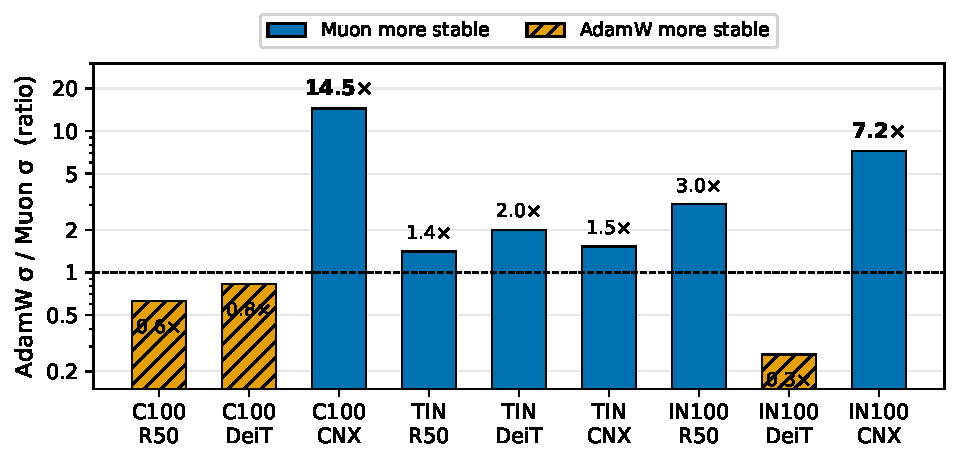
\includegraphics[width=\textwidth]{figures/fig3_stability.pdf}
\caption{Cross-seed standard deviation ($\sigma$) for Muon vs AdamW across all nine settings. Muon exhibits lower variance on 6/9 configurations; the stability advantage is architecture-dependent.}
\label{fig:stability}
\end{figure}

Cross-seed variance is architecture-dependent (Figure~\ref{fig:stability}): Muon shows substantially lower variance on convolutional architectures ($\sigma{=}0.15$ vs.\ $2.17$ on ConvNeXt-T/CIFAR-100), but AdamW is more stable on DeiT-S/ImageNet-100 ($\sigma{=}0.10$ vs.\ $0.38$).
Where Muon's variance reduction exceeds $7\times$ (ConvNeXt-T), fewer seeds suffice for reliable estimates.

% =============================================================================
% Appendix: Metric Robustness
% =============================================================================
\section{Metric Robustness}\label{sec:metric_robustness}

The sign reversal reported in Section~\ref{sec:spectral_analysis} is not an artifact of the chosen spectral metric. We verify this by computing the Spearman correlation between per-layer Muon benefit $\Delta a_l$ and three alternative divergence measures:

\begin{table}[h]
\centering
\caption{Spearman $\rho$ between per-layer divergence and Muon benefit under three spectral metrics. The sign reversal (positive on ResNet-50, negative on DeiT-S) is consistent across all metrics.}
\label{tab:metric_robustness}
\small
\begin{tabular}{@{}lcccc@{}}
\toprule
Metric & \multicolumn{2}{c}{ResNet-50} & \multicolumn{2}{c}{DeiT-S} \\
\cmidrule(lr){2-3} \cmidrule(lr){4-5}
 & $\rho$ & $p$ & $\rho$ & $p$ \\
\midrule
$\Delta\mathrm{sr}_l$ (stable rank) & $+0.45$ & ${<}0.001$ & $-0.40$ & $0.004$ \\
FCSB margin & $+0.40$ & ${<}0.01$ & $-0.51$ & ${<}0.001$ \\
$\Delta\mathrm{er}_l$ (effective rank) & $+0.43$ & ${<}0.01$ & $-0.33$ & $0.02$ \\
\bottomrule
\end{tabular}
\end{table}

All three metrics yield positive correlations on ResNet-50 and negative correlations on DeiT-S, confirming that the sign reversal is a robust structural phenomenon independent of the specific spectral measure.
We adopt stable rank as the primary metric because it is the most conservative (smallest $|\rho|$ on DeiT-S) and has favorable analytical properties: it is bounded, well-defined for rank-deficient matrices, and requires no architecture-specific normalization.

% =============================================================================
% Appendix: Normalization Swap Details
% =============================================================================
\section{Normalization Swap Implementation}\label{sec:normswap_details}

We replace all BatchNorm2d layers in ResNet-50 with GroupNorm(1, $C$), where $C$ is the number of channels.
GroupNorm with a single group computes statistics over all spatial and channel dimensions of each sample independently, making it equivalent to LayerNorm applied to convolutional feature maps~\cite{wu2018group}.
This substitution replaces 53 BatchNorm layers; all other architecture parameters, hyperparameters, and the training protocol remain identical to the standard ResNet-50 experiments (Section~\ref{sec:experimental_setup}).

% =============================================================================
% Appendix: Ablation Details
% =============================================================================
\section{Parameter Grouping Ablation Details}\label{sec:ablation_details}

The two-group AdamW ablation mirrors Muon's parameter routing exactly: 53 two-dimensional weight matrices ($23.45$M parameters, $\text{lr}{=}10^{-3}$) and 108 one-dimensional parameters ($0.26$M parameters, $\text{lr}{=}3{\times}10^{-4}$), with AdamW applied to both groups.
On ResNet-50 (CIFAR-100), two-group AdamW achieves $66.36 \pm 0.40\%$ ($n{=}3$, seeds 42/2/3), comparable to single-group AdamW ($67.85 \pm 0.17\%$) and far below Muon ($76.88 \pm 0.27\%$).
On ConvNeXt-T, two-group AdamW similarly matches standard AdamW ($59.44 \pm 0.28\%$ vs.\ $58.54 \pm 2.17\%$) while Muon maintains a $+15.2$\,pp advantage ($74.62 \pm 0.15\%$).
On DeiT-S, two-group AdamW degrades catastrophically to $30.08\%$ ($-22.3$\,pp vs.\ standard AdamW, single seed), as the reduced learning rate for 1D parameters (104/152 tensors in DeiT-S) severely undertrained LayerNorm parameters.

% =============================================================================
% Appendix I: Architecture Coverage Rationale
% =============================================================================
\section{Architecture Coverage in Supplementary Experiments}\label{sec:arch_coverage}

% =============================================================================
% Appendix: Additional Optimizer Comparisons
% =============================================================================
\section{Additional Optimizer Comparisons}\label{sec:additional_optimizers}

We evaluated Lion~\cite{chen2024lion} as a representative of sign-based optimizers to verify that the spectral family's advantage is not shared by all non-Adam methods.
On ResNet-50/CIFAR-100, Lion achieves $69.42\%$ (vs.\ AdamW $67.85\%$, $+1.57$\,pp), far below the spectral family ($+9$--$+10$\,pp over AdamW), confirming that the advantage is specific to spectral preconditioning rather than a general property of non-diagonal methods.
Other recent optimizers---Sophia~\cite{liu2024sophia} (diagonal Hessian clipping), Prodigy~\cite{mishchenko2024prodigy} (learning-rate-free estimation), GaLore~\cite{zhao2024galore} (low-rank gradient projection)---target computational cost or tuning difficulty rather than architecture robustness, making them complementary to rather than competitors of spectral methods.
A comprehensive comparison with these methods is left to future work.

% =============================================================================
% Appendix I: Architecture Coverage Rationale
% =============================================================================
\section{Architecture Coverage in Supplementary Experiments}\label{sec:arch_coverage}

The extended experiments in Appendix~\ref{sec:alt_spectral} focus on ResNet-50 and ConvNeXt-T rather than all three architectures from the main experiments. These two architectures represent the extremes of the normalization spectrum that drives Muon's variable effectiveness: ResNet-50 uses BatchNorm, where Muon's spectral updates interact with the implicit conditioning provided by BN; ConvNeXt-T uses LayerNorm, where the Muon--AdamW gap is largest (up to +24.30\,pp on IN100 at 20 epochs). DeiT-S, which also uses LayerNorm but in a pure self-attention architecture, exhibits intermediate gap magnitudes and is already thoroughly characterized across three datasets, three seed replicates, and two training horizons (20 and 50 epochs) in the main paper. Including DeiT-S in the supplementary experiments would add six additional training runs without meaningfully extending the analysis beyond the BN--LN axis already captured by the ResNet-50/ConvNeXt-T pair.

\section{Corruption Robustness}\label{sec:corruption_robustness}

We evaluate corruption robustness on CIFAR-100-C~\cite{hendrycks2019benchmarking}, which applies 19 corruption types at 5 severity levels to the CIFAR-100 test set. We report mean corruption error (mCE), normalized so that same-architecture, same-normalization AdamW = 100\%; lower is better.

\begin{table}[h]
\centering
\caption{Corruption robustness on CIFAR-100-C. mCE ($\downarrow$ is better) normalized so same-normalization AdamW = 100\%. Retention = corruption accuracy\,/\,clean accuracy, measuring inherent robustness independent of clean performance level.}
\label{tab:corruption_robustness}
\small
\begin{tabular}{llcccc}
\toprule
Architecture & Optimizer & Clean Acc (\%) & Corr Acc (\%) & mCE (\%) & Retention (\%) \\
\midrule
\multirow{4}{*}{ResNet-50 (BN)} & SOAP & 77.28 & 22.74 & \textbf{98.6} & 29.4 \\
 & Shampoo & 78.25 & 21.94 & 99.8 & 28.0 \\
 & AdamW & 67.85 & 22.40 & 100.0 & 33.0 \\
 & Muon & 76.88 & 21.59 & 100.5 & 28.1 \\
\midrule
\multirow{2}{*}{ResNet-50 (LN)} & Muon & 78.52 & 27.44 & \textbf{92.6} & 34.9 \\
 & AdamW & 50.51 & 22.93 & 100.0 & 45.4 \\
\midrule
\multirow{4}{*}{ConvNeXt-T} & Muon & 74.62 & 31.31 & \textbf{90.5} & 42.0 \\
 & SOAP & 74.40 & 26.23 & 99.1 & 35.3 \\
 & AdamW & 58.54 & 26.23 & 100.0 & 44.8 \\
 & Shampoo & 70.57 & 23.55 & 103.9 & 33.4 \\
\midrule
\multirow{4}{*}{DeiT-S} & Muon & 62.67 & 28.30 & \textbf{89.2} & 45.2 \\
 & SOAP & 65.45 & 21.47 & 98.3 & 32.8 \\
 & AdamW & 52.33 & 20.89 & 100.0 & 39.9 \\
 & Shampoo & 63.53 & 18.77 & 102.6 & 29.5 \\
\midrule
\multirow{5}{*}{ResNet-50 (GN32)} & Muon & 78.20 & 28.75 & \textbf{90.0} & 36.8 \\
 & SOAP & 75.52 & 27.88 & 91.3 & 36.9 \\
 & Shampoo & 74.79 & 26.96 & 92.6 & 36.0 \\
 & AdamW & 55.73 & 22.58 & 100.0 & 40.5 \\
 & SGD & 23.90 & 14.36 & 112.9 & 60.1 \\
\bottomrule
\end{tabular}
\end{table}

Muon achieves the lowest mCE on three of four architecture configurations (ConvNeXt-T: 90.5\%, DeiT-S: 89.2\%, ResNet-50-LN: 92.6\%), with the robustness advantage most pronounced on layer-normalized architectures. On ResNet-50 with BatchNorm, differences among optimizers are marginal (mCE 98.6--100.5\%), consistent with BatchNorm's known loss-landscape smoothing effect. Shampoo underperforms AdamW on ConvNeXt-T (mCE 103.9\%) and DeiT-S (102.6\%), while performing near-baseline on ResNet-50-BN (99.8\%), indicating that full-matrix Kronecker preconditioning does not translate to corruption robustness. Category-level analysis reveals that Muon's advantage concentrates in weather and digital corruptions (brightness, saturate, snow, frost, spatter), while noise corruptions (Gaussian, shot, impulse) show smaller inter-optimizer differences.

\paragraph{Dose-response pattern in corruption robustness.}
The GN(32) configuration extends the dose-response pattern observed in clean accuracy (Section~\ref{sec:norm_swap}) to corruption robustness. Under GN(32), all three spectral optimizers improve mean corruption accuracy by 5--7\,pp relative to their BN counterparts (Muon: $+7.2$\,pp, SOAP: $+5.1$\,pp, Shampoo: $+5.0$\,pp), while AdamW remains flat ($+0.2$\,pp). SGD under GN(32) degrades to 14.36\% mean corruption accuracy (mCE 112.9\%), an 8.2\,pp drop below GN(32) AdamW, mirroring the clean-accuracy collapse observed in the normalization-swap experiment. This three-way divergence---spectral methods improve, AdamW holds steady, SGD degrades---constitutes a dose-response pattern: as normalization smoothing is reduced from BN to GN(32), the optimizer's capacity for spectral preconditioning determines whether it can compensate for the lost implicit conditioning, in corruption robustness as in clean accuracy.


\end{document}
